\documentclass[12pt]{extarticle}
\usepackage{geometry}
\geometry{
a4paper,
total={170mm,257mm},
left=20mm,
top=20mm,
headheight=12pt
}

\usepackage[parfill]{parskip} % Activate to begin paragraphs with an empty line rather than an indent
\usepackage{graphicx} % Use pdf, png, jpg, or eps§ with pdflatex; use eps in DVI mode
% TeX will automatically convert eps --> pdf in pdflatex
\graphicspath{ {../Figures/} }
\usepackage[labelfont=bf]{caption}
\usepackage{float}

\usepackage{amssymb,amsmath,amsthm}
\usepackage{commath}
\usepackage[hyphens]{url}
\usepackage[dvipsnames]{xcolor}
\usepackage[unicode=true,colorlinks=true,urlcolor=CadetBlue,citecolor=black,linkcolor=black]{hyperref}
\PassOptionsToPackage{hyphens}{url} % url is loaded by hyperref
\usepackage{authblk}
\usepackage{longtable}
\usepackage{multirow}
\usepackage{booktabs}
\usepackage{lipsum}  
\usepackage[title,page]{appendix}
\usepackage{chngcntr}
%\usepackage{endfloat}
      
%SetFonts
% newtxtext+newtxmath
\usepackage{newtxtext} %loads helv for ss, txtt for tt
\usepackage{amsmath}
\usepackage[bigdelims]{newtxmath}
\usepackage[T1]{fontenc}
\usepackage{textcomp}
%SetFonts

% Line Spacing 
\linespread{1.25}
    
% Species names
%% Meta-Command for defining new species macros
\usepackage{xspace}

\newcommand{\species}[3]{%
  \newcommand{#1}{\gdef#1{\textit{#3}\xspace}\textit{#2}\xspace}}
  
\species{\yeast}{Saccharomyces cerevisiae}{S.~cerevisiae}
\species{\calbicans}{Candida albicans}{C.~albicans}
\species{\cneoformans}{Cryptococcus neoformans}{C.~neoformans}

% line numbers
\usepackage[displaymath, mathlines]{lineno}
\renewcommand\linenumberfont{\normalfont\small\sffamily}
\linenumbers
\modulolinenumbers[2]

% Yoav & Lee commands
\newcommand*{\tr}{^\intercal}
\let\vec\mathbf
\newcommand{\matrx}[1]{{\Big[ \stackrel{}{#1}\Big]}}
\newcommand{\diag}[1]{\mbox{diag}\matrx{#1}}
\newcommand{\goesto}{\rightarrow}
\newcommand{\dspfrac}[2]{\frac{\displaystyle #1}{\displaystyle #2} }
\newtheorem{theorem}{Theorem}
\newtheorem{corollary}{Corollary}
\newtheorem{lemma}{Lemma}
\newtheorem{remark}{Remark}
\newtheorem{result}{Result}
\renewcommand\qedsymbol{} % no square at end of proof
\newcommand{\cl}{\mathbf{L}}
\newcommand{\cj}{\mathbf{J}}
\newcommand{\ci}{\mathbf{I}}
\DeclareMathOperator{\sign}{sign}

% Supplementary
% https://support.authorea.com/en-us/article/how-to-create-an-appendix-section-or-supplementary-information-1g25i5a/
\newcommand{\beginsupplement}{%
      	\setcounter{table}{0}
        \renewcommand{\thetable}{S\arabic{table}}%
        \setcounter{figure}{0}
        \renewcommand{\thefigure}{S\arabic{figure}}%
		\setcounter{equation}{0}
        \renewcommand{\theequation}{A\arabic{equation}}%
}

% autoref
\def\equationautorefname{Eq.}

% NatBib
\usepackage[numbers,square,comma,sort]{natbib}

% Title page
\title{Non-Vertical Cultural Transmission, Assortment, \\and the Evolution of Cooperation}

\date{\today}

\begin{document}
\maketitle


\pagebreak
{\large This work was carried out under the supervision of \textbf{Dr. Yoav Ram} from the Efi Arazi School of Computer Science, The Interdisciplinary Center, Herzliya.}
\pagebreak

{\huge \begin{center} \textbf{Abstract} \end{center}}

Cultural evolution of cooperation under vertical and non-vertical cultural transmission is studied, and conditions are found for fixation and coexistence of cooperation and defection. 
The evolution of cooperation is facilitated by its horizontal transmission and by an association between social interactions and horizontal transmission.
The effect of oblique transmission depends on the horizontal transmission bias.
Stable polymorphism of cooperation and defection can occur, and
when it does, reduced association between social interactions and horizontal transmission evolves, which leads to a decreased frequency of cooperation and lower population mean fitness.
The deterministic conditions are compared to outcomes of stochastic simulations of structured populations.
Parallels are drawn with Hamilton's rule incorporating relatedness and assortment.

\pagebreak

\tableofcontents
\pagebreak


%%%%%%%%%%%%%%%%%%%%%%%%%%%%%%%%%%%%%%%%%%%%%%%%%%%%%%
%%% Introduction
\section{Introduction}
Cooperative behavior can reduce an individual's fitness and increase the fitness of its conspecifics or competitors~\citep{axelrod1981evolution}.
Nevertheless, cooperative behavior appears to occur in many animals~\citep{dugatkin1997cooperation}, including humans, primates~\citep{jaeggi2013natural},  rats~\citep{rice1962altruism}, birds~\citep{stacey1990cooperative,krams2008experimental}, and lizards~\citep{sinervo2006self}.
Evolution of cooperative behavior has been an important focus of research in evolutionary theory since at least the 1930s~\citep{Haldane1932book}.
Since the work of  \citet{hamilton1964genetical} and \citet{axelrod1981evolution}, theories for the evolution of cooperative and altruistic behaviors have been intertwined often under the rubric of \emph{kin selection}.
Kin selection theory posits that natural selection is more likely to favor cooperation between more closely related individuals.
The importance of \emph{relatedness} to the evolution of cooperation and altruism was demonstrated by \citet{hamilton1964genetical}, who showed that an allele that determines cooperative behavior will increase in frequency if the reproductive cost to the actor that cooperates, $c$, is less than the benefit to the recipient, $b$, times the relatedness, $r$, between the recipient and the actor.
This condition is  known as \emph{Hamilton's rule}:
\begin{equation} \label{eq:hamilton_rule}
c < b \cdot r,
\end{equation}
where the relatedness coefficient $r$ measures the probability that an allele sampled from the cooperator is identical by descent to one at the same locus in the recipient.

There is an ongoing debate about to what extent kin selection explains evolution of cooperation and altruism.
It has been suggested that kin selection to explain the cooperative behaviour of eusocial insects like the honey bee.
The most significant argument against kin selection is that cooperation can evolve with zero relatedness \cite{wilson2005kin}. This makes Hamilton's rule incomplete according to Wilson \cite{wilson2005kin}. Foster et al. \cite{foster2006kin} reject this claim. 
They argue that altruism without relatedness can not evolve. They refer us to Hamilton who claimed that relatedness can arise without recent common ancestry. 
Wilson also criticises kin selection on the grounds that environmental or ecological factors probably be more important than relatedness in determining social actions. On the other hand, Foster et al. \cite{foster2006kin} argue that kin selection does not ignore ecology. 
Hamilton’s rule shows that environmental factors causing a high benefit: cost ratio will favour cooperation.

Beside kin selection, two more major theroies were suggested to explain to evolution of cooperation.

\textbf{Reciprocity} suggests repeating interactions or individual recognition as key factors for explaining the evolution of cooperation. 
In \textit{direct reciprocity} there are a repeated encounters between the same two individuals. In every encounter, each player has a choice between cooperation and defection. If I cooperate now, you may cooperate later. Hence, it may pay off to cooperate.
This game-theoretic framework is known as the repeated Prisoner's Dilemma. 
Direct reciprocity can only lead to the evolution of cooperation if the cost is smaller than $w$ the probability for another encounter between the same two individuals multiplied by the benefit. 
\begin{equation} \label{reciprocity}
c<bw
\end{equation}
Direct reciprocity assumes that both players are in a position to cooperate. Direct reciprocity can not explain cooperation in asymmetric interactions. In humans, such interactions happen often, for example humans often donate money. 
\textit{Indirect reciprocity} has been suggested to explain this behavior. 
Nowak \cite{nowak2006five} claims that direct reciprocity is like a barter economy based on the immediate exchange of goods, while indirect reciprocity resembles the invention of money. The money that "fuels the engines" of indirect reciprocity is reputation. 
However, Reciprocity assume repeating interactions and therefore, has difficulty explaining evolution of cooperation if the no repeating interactions occurs. 

\textbf{Group Selection} theory posits that cooperation is favoured because of the advantage to the whole group, if selection acts at the group level in addition to the individual level. A common model for group selection work as is: the population is divided into groups. In each groups there are cooperators, which help to other group members and defectors which do not help. 
Individuals reproduce proportional to their fitness. Offspring are added to the same group.
If a group reaches a certain size it can split to two groups. A group that grow faster will split more often. Groups of cooperators are growing faster than group of defectors.
Therefore, cooperation can evolve in this model when the ratio between benefit b and cost c is more than one plus the ratio between the maximum group size n and the number of groups m:
\begin{equation} \label{groupselection}
\frac{b}{c}>1+\frac{n}{m}
\end{equation}


All three theories mentioned above assume that cooperation is genetically determined. This raise the question, is it possible that cooperation is determined by environmental or social influences.
Cooperative behavior can be subject to \emph{cultural transmission}, which allows an individual to acquire attitudes or behavioral traits from other individuals in its social group through imitation, learning, or other modes of communication \citep{cavalli1981cultural,richerson2008not}.
Cultural transmission may be  modeled as vertical, horizontal, or oblique:  vertical transmission occurs between parents and offspring, horizontal transmission occurs between individuals from the same generation, and oblique transmission occurs  to offspring from the generation to which their parents belong (i.e. from non-parental adults). 
Evolution under either of these transmission models can be be more rapid than under pure vertical transmission~\citep{cavalli1981cultural,lycett2008questions,ram2018evolution}.

Here, we study models for the cultural evolution of cooperation that include both vertical and non-vertical transmission. 
%We investigate these models using mathematical analysis and simulations.  
In our models behavioral changes are mediated by cultural transmission that can occur specifically during social interactions.
For instance, there may be an association between the choice of partner for social interaction and the choice of partner for cultural transmission,
or when an individual interacts with an individual of a different phenotype,  exposure to the latter may lead the former to  convert its phenotype.
Our results demonstrate that cultural transmission, when associated with social interactions, can enhance the evolution of cooperation even when genetic transmission cannot, partly because it facilitates the generation of assortment \citep{Fletcher2009assortment}, and partly because it diminishes the effect of selection (due to non-vertical transmission from non-reproducing individuals~\citep{ram2018evolution}).

To understand the evolution of cooperation we are going to use \emph{replicator dynamics}. The replicator in replicator dynamics has the ability to make one or more copies of itself.
The replicator can be a gene, a phenotype, a stragey in a game and etc. In cooperation context replicator is a different stragey in the game, whether the individual is a cooperative or a defector.
In replicator dynamics we assume large population of replicators, which interact with respect to their proportion.
Those interactions of different replicator affect the fitness acorrding to some payoff matrix. The payoff matrix depands on the game which is played. 
The most common game to describe cooperation is prisoner's dilemma\citep{nowak1992tit}.
Similar to dominant strategies bringing forth Nash equilibria when games are repeated, strategies in replicator dynamics can become evolutionary stable. Such strategies are called \emph{Evolutionarily Stable stragey (ESS)}.
Such strategies cannot be invaded by any other strategy that is initially rare. 
One of the main questions in the evolution of cooperation is under what conditions such invasions are possible.

\newpage
\section{Related Work}

\citet{Eshel1982} studied a related model for the evolution of cooperative behavior.
Their model included \emph{assortative meeting}, or non-random encounters, where a fraction $m$ of individuals in the population each interact specifically with an individual of the same phenotype, and a fraction $1-m$ interacts  with a randomly chosen individual.  
Such assortative meeting may be due, for example, to population structure or active partner choice.
In their model, cooperative behavior can evolve if
\citep[eq.~3.2]{Eshel1982}
\begin{equation} \label{eq:eshel1982}
c < b \cdot m \,,
\end{equation}
where $b$ and $c$ are the benefit and cost of cooperation\footnote{In an extended model, which allows an individual to encounter $N$ individuals before choosing a partner, the right hand side is multiplied by $E[N]$, the expected number of encounters \citep[eq.~4.6]{Eshel1982}.
}. 

The role of assortment in the evolution of altruism was emphasized by \citet{Fletcher2009assortment}.
They found that in a \emph{public-goods} game, altruism will evolve if cooperative individuals experience more cooperation, on average, than defecting individuals, and ``thus, the evolution of altruism requires (positive) assortment between focal \emph{cooperative} players and cooperative acts in their interaction environment.''
With some change in parameters, this condition is summarized by \citep[eq.~2.3]{Fletcher2009assortment}
\begin{equation} \label{eq:fletcher2009}
c < b \cdot (p_C - p_D ) \,,
\end{equation}
where $p_C$ is the probability that a cooperator receives help, and $p_D$ is the probability that a defector receives help\footnote{Inequality~\ref{eq:fletcher2009} generalizes inequalities~\ref{eq:hamilton_rule} and~\ref{eq:eshel1982} by substituting $p_C=r + p$, $p_D=p$ and $p_C=m + (1-m)p$, $p_D=(1-m)p$, respectively, where $p$ is the frequency of cooperators.}.
\citet{Bijma2010assortment} obtained a result related to inequality~\ref{eq:fletcher2009} for other games.

Cooperation can also evolve when interactions are determined by population structure. For example, \citet{Ohtsuki2006} studied populations on graphs with average degree $k$, that is, the average individual has $k$ potential interaction partners. Assuming that selection is weak and that the population size is much larger than $k$ (i.e. sparse structure), they found that cooperative behaviour can evolve if~\citep{Ohtsuki2006}
\begin{equation} \label{eq:ohtsuki2006}
c < b \cdot \frac{1}{k} \,.
\end{equation}
They thus interpret $1/k$ as \emph{social relatedness} or \emph{social viscosity}~\citep{Ohtsuki2006}.


\citet{feldman1985gene} introduced the first model for the evolution of altruism by cultural transmission with kin selection and demonstrated that if the fidelity of cultural transmission of altruism is $\varphi$, then the condition for evolution of altruism in the case of sib-to-sib altruism is \citep[Eq.~16]{feldman1985gene}
\begin{equation} \label{eq:feldman1985}
c < b \cdot \varphi - \frac{1-\varphi}{\varphi} \,.
\end{equation}
In inequality~\ref{eq:feldman1985}, $\varphi$ replaces relatedness ($r$ in inequality~\ref{eq:hamilton_rule}) or assortment ($m$ in inequality~\ref{eq:eshel1982}), but the effective benefit $b\cdot \varphi$ is  reduced by $(1-\varphi)/\varphi$.
This shows that under a cultural transmission, the condition for the evolutionary success of altruism entails a modification of Hamilton's rule (inequality~\ref{eq:hamilton_rule}).

Both \citet{woodcock2006significance} and \citet{lewin2017microbes} demonstrated that non-vertical transmission can help explain the evolution of cooperative behavior, the former using simulations with cultural transmission, the latter using a model where cooperation is mediated by host-associated microbes.
Indeed, models in which microbes affect their host's behavior~\citep{lewin2017microbes,lewin2020rockpaperscissors,gurevich2020parental} are mathematically similar to models of cultural transmission, and they also emphasize the role of non-vertical transmission~\citep{cavalli1981cultural}.

\citet{handley2020human} showed the importance of culture on the human behavior. They showed that the probablity of indvidual to cooperate with unrelated strangers from a different group in transient interactions corresponds to the degree of cultural similarity between those groups.
Therefore, they have suggested that group-level selection on culturally differentiated populations can explain cooperation between unrelated humans from different groups.

%%%%%%%%%%%%%%%%%%%%%%%%%%%%%%%%%%%%%%%%%%%%%%%%%%%%%%
% Models
\newpage
\section{Models}

Consider a large population whose members can be one of two phenotypes: $\phi=A$ for cooperators or $\phi=B$ for defectors.
An offspring inherits its phenotype from its parent via vertical transmission with probability $v$ or from a random individual in the parental population via oblique transmission with probability $(1-v)$ (\autoref{fig:illustration}a). 
Following~\citet{ram2018evolution}, given that the parent's phenotype is $\phi$ and assuming uni-parental inheritance~\citep{Zefferman2016}, the conditional probability that the phenotype $\phi'$ of the offspring is $A$ is 
\begin{equation} \label{eq:vertical_oblique_transmission}
P(\phi'=A \mid \phi) = \begin{cases}
v + (1-v)p, & \text{if } \phi=A \\
(1-v)p, & \text{if } \phi=B
\end{cases},
\end{equation}
where $p=P(\phi=A)$ is the frequency of $A$ among all adults in the parental generation.  

Not all adults become parents, and we denote the frequency of phenotype $A$ among parents by $\dot{p}$.
Therefore, the frequency $\hat{p}$ of  phenotype $A$ among juveniles (after selection and vertical and oblique transmission) is
\begin{equation}\label{eq:horizontal}
\begin{aligned}
\hat{p} \;=
\dot{p} [v + (1-v)p] + (1-\dot{p}) [(1-v)p] \;= 
v \dot{p} + (1-v) p \;.
\end{aligned}
\end{equation}
Individuals are assumed to interact according to a \emph{prisoner's dilemma}.
Specifically, individuals interact in pairs; a cooperator suffers a fitness cost $0<c<1$, and its partner gains a fitness benefit $b$, where we assume $c<b$. \autoref{fig:illustration}a shows the payoff matrix, i.e. the fitness of an individual with phenotype $\phi_1$ when interacting with a partner of phenotype $\phi_2$.
The choise of prisoner's dilemma as the interaction model was motividated by the fact that prisoner's dilemma is a common game used to study evolution of cooperation\citep{axelrod1981evolution}, \citep{milinski1987tit}, \citep{nowak1992tit}.
Although we decided to focus on prisoner's dilemma, other games such as stag hunt\citep{skyrms2004stag} may be a better explaination of cooperation behavior in humman\citep{tomasello2012two}.

%%% Figure: model illustration
\begin{figure}[pt]
  \centering
  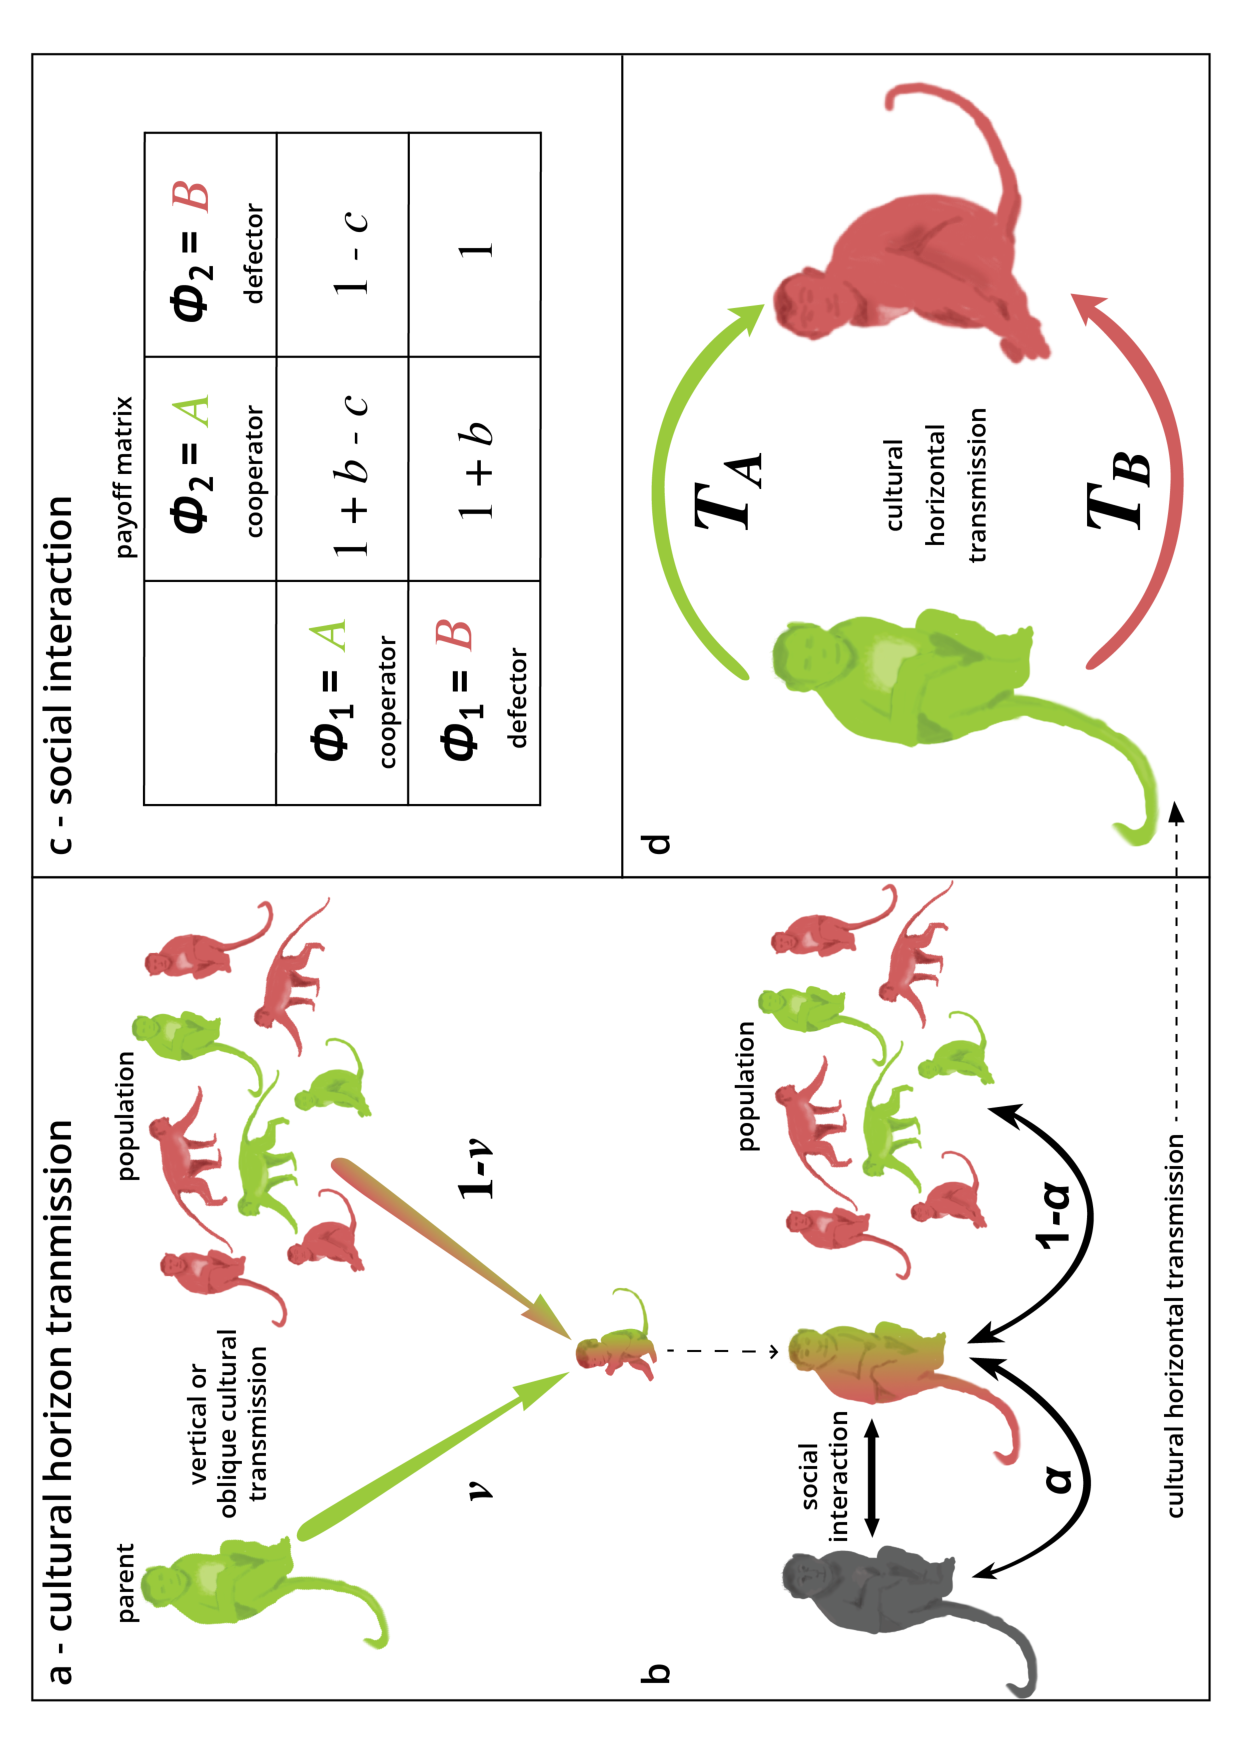
\includegraphics[width=0.7\textwidth]{../PRSB_figures/fig_1.pdf}
  \caption{\textbf{Model illustration.} 
  \textbf{(a)}~First, offspring inherit their parent's phenotype via vertical cultural transmission with probability $v$, or the phenotype of a random non-parental adult via oblique cultural transmission with probability $1-v$.
  \textbf{(b)}~Second, adults socially interact in pairs in a prisoner's dilemma game. Horizontal cultural transmission occurs from a random individual in the population, with probability $1-\alpha$, or from the social partner, with probability $\alpha$, where $\alpha$ is the interaction-transmission association parameter.
  \textbf{(c)}~The prisoner's dilemma payoff matrix shows the fitness of phenotype $\phi_1$ when interacting with phenotype $\phi_2$.
    \textbf{(d)}~The probabilities of successful horizontal cultural transmission of phenotypes $A$ (cooperator) and $B$ (defector) are $T_A$ and $T_B$, respectively.
    }
  \label{fig:illustration}
\end{figure}


Social interactions occur randomly:
two juvenile individuals with phenotype $A$ interact with probability~$\hat{p}^2$, two juveniles with phenotype $B$ interact with probability $(1-\hat{p})^2$, and two juveniles with different phenotypes interact with probability $2\hat{p}(1-\hat{p})$. 
Horizontal cultural transmission occurs between pairs of individuals from the same generation. 
It occurs between socially interacting partners with probability~$\alpha$, or between a random pair with probability~$1-\alpha$ (see~\autoref{fig:illustration}b).
%The interaction-transmission association $\alpha$ is therefore the fraction of population that receives (horizontal transmission) from the social interaction partner, and $1-\alpha$ receives randomly.
However, horizontal transmission is not always successful, as one partner may reject the other's phenotype.
The probability of successful horizontal transmission of phenotypes $A$ and $B$ are $T_A$ and $T_B$, respectively (\autoref{table:interactions}, \autoref{fig:illustration}d).
Thus, the frequency $p'$ of phenotype $A$ among adults in the next generation, after horizontal transmission, is 
\begin{equation}\label{eq:nextgen_adults}
\begin{aligned}
p' \;= \;
& \hat{p}^2 \big[\alpha + (1-\alpha)\big(\hat{p} + (1-\hat{p})(1-T_B)\big)\big] \;+ \\
& \hat{p}(1-\hat{p}) \big[\alpha(1-T_B) + (1-\alpha)\big(\hat{p} + (1-\hat{p})(1-T_B)\big)\big] \;+ \\
& (1-\hat{p})\hat{p} \big[\alpha T_A + (1-\alpha) \hat{p} T_A \big] \;+ 
(1-\hat{p})^2 \big[(1-\alpha) \hat{p} T_A \big] \\
=\; & \hat{p}^2(T_B-T_A) \;+\; \hat{p}(1+T_A-T_B) \;.
\end{aligned}
\end{equation}
The frequency of $A$ among parents (i.e. after selection) follows a similar dynamic, but also includes the effect of natural selection, and is therefore
\begin{equation}\label{eq:nextgen_parents}
\begin{aligned}
\bar{w} \dot{p}' =
& \hat{p}^2 (1+b-c) \big[\alpha + (1-\alpha)\big(\hat{p} + (1-\hat{p})(1-T_B)\big)\big] \;+ \\
& \hat{p}(1-\hat{p}) (1-c) \big[\alpha(1-T_B) + (1-\alpha)\big(\hat{p} + (1-\hat{p})(1-T_B)\big)\big] \;+ \\
& (1-\hat{p})\hat{p} (1+b) \big[\alpha T_A + (1-\alpha) \hat{p} T_A \big] \;+\; 
(1-\hat{p})^2 \big[(1-\alpha) \hat{p} T_A \big] \;,
\end{aligned}
\end{equation}
where fitness values are taken from \autoref{fig:illustration}c and \autoref{table:interactions}, and the population mean fitness is
$\bar{w} =  1 + \hat{p}(b-c)$.
Starting from \autoref{eq:horizontal} with $\hat{p}'=v\dot{p}'+(1-v)p'$, we substitute $p'$ from \autoref{eq:nextgen_adults} and $\dot{p}'$ from \autoref{eq:nextgen_parents} and obtain
\begin{equation} \label{eq:nextgen_juveniles}
\begin{aligned}
\hat{p}' =
& \frac{v}{\bar{w}}\Big[\hat{p}^2(1+b-c)\Big(1-(1-\hat{p})(1-\alpha)T_B)\Big)\Big] \;+ \\
& \frac{v}{\bar{w}}\Big[ \hat{p}(1-\hat{p})(1-c)\big( \hat{p}(1-\alpha)T_B + 1 - T_B \big) \Big] \;+ \\
& \frac{v}{\bar{w}}\Big[ \hat{p}(1-\hat{p})(1+b)\big(\hat{p}(1-\alpha) + \alpha \big) T_A \Big] \;+ \\
& \frac{v}{\bar{w}}(1-\hat{p})^2\hat{p}(1-\alpha)T_A \;+\;
(1-v)\hat{p}^2(T_B-T_A) \;+\;
(1-v)\hat{p}(1+T_A-T_B) \;.
\end{aligned}
\end{equation}
\autoref{table:vars_params} lists the model variables and parameters.

%%% Table: variables and parameters
%%%% Table
\begin{table}[p]
  \caption{\textbf{Interaction frequency, fitness, and transmission probabilities.}}
  \begin{tabular}{@{}llllll@{}}
  \toprule
  \multirow{2}{*}{Phenotype $\phi_1$} &
    \multirow{2}{*}{Phenotype $\phi_2$} &
    \multirow{2}{*}{Frequency} &
    \multirow{2}{*}{Fitness of $\phi_1$} &
    \multicolumn{2}{l}{$P(\phi_1=A)$ via horizontal transmission:} \\ \cmidrule(l){5-6} 
      &     &                      &         & from partner, $\alpha$ & from population, $(1-\alpha)$ \\ \cmidrule(r){1-6}
  $A$ & $A$ & $\hat{p}^2$          & $1+b-c$ & 1                      & $\hat{p}+(1-\hat{p})(1-T_B)$  \\
  $A$ & $B$ & $\hat{p}(1-\hat{p})$ & $1-c$   & $1-T_B$                & $\hat{p}+(1-\hat{p})(1-T_B)$  \\
  $B$ & $A$ & $\hat{p}(1-\hat{p})$ & $1+b$   & $T_A$                  & $\hat{p} T_A$                 \\
  $B$ & $B$ & $(1-\hat{p})^2$      & $1$     & $0$                    & $\hat{p} T_A$                 \\ \bottomrule
  \end{tabular}
  \label{table:interactions}
\end{table}
\bigskip

\begin{table}[p]
\centering
\caption{\textbf{Model variables and parameters.}
}
\begin{tabular}{lll}
\toprule
Symbol & Description & Values \\ \cmidrule(r){1-3}
$A$ & Cooperator phenotype & \\
$B$ & Defector phenotype & \\
$p$ & Frequency of phenotype $A$ among adults & $[0,1]$ \\
$\dot p$ & Frequency of phenotype $A$ among parents & $[0,1]$ \\
$\hat p$ & Frequency of phenotype $A$ among juveniles & $[0,1]$ \\
$v$ & Vertical transmission rate & $[0,1]$ \\
$c$ & Cost of cooperation & $(0,1)$ \\
$b$ & Benefit of cooperation & $c<b$ \\
$\alpha$ & Probability of interaction-transmission association & $[0,1]$ \\
$T_A, T_B$ & Horizontal transmission rates of phenotype $A$ and $B$ & $(0,1)$ \\
\\ \bottomrule
\end{tabular}
\label{table:vars_params}
\end{table}

\newpage
%%%%%%%%%%%%%%%%%%%%%%%%%%%%%%%%%%%%%%%%%%%%%%%%%%%%%%
%%% Results
\newpage
\section{Results}

We determine the equilibria of the model in \autoref{eq:nextgen_juveniles}
and analyze their local stability.
We then analyze the evolution of a modifier of interaction-transmission association,~$\alpha$.
Finally, we compare derived conditions to outcomes of stochastic simulations with a structured population.

%%%%%%%%%%%%%%%%%%%%%%%%%%%%%%%%%%%%%%%%%%%%%%%%%%%%%%
\subsection{Evolution of cooperation}

To learn about the evolution of cooperation we investigate local stability of the equilibria of the model in \autoref{eq:nextgen_juveniles}.
The equilibria are the solutions of $\hat{p}'-\hat{p}=0$. Note that \autoref{eq:nextgen_juveniles} may look simple cubic polynomial. However, because $\bar{w}$ is a function of $\hat{p}$, \autoref{eq:nextgen_juveniles} is not simple polynomial but a fractional polynomial. 
The solution of fractional polynomial is not trivial and that is why it is better to find the equilibria and analyze the stability.
The fixed points (equilibria) of the recursion (\autoref{eq:nextgen_juveniles}) are $\hat p=0$, $\hat p=1$, and (see Appendix~\ref{sec:appendixB} \autoref{eq:general_equilibrium_appendix})
\begin{equation} \label{eq:general_equilibrium}
  \hat{p}^* =  
  \frac{\alpha bvT_A - cv(1-T_B) + (T_A-T_B)}{\big[c(1-v) - b (1-\alpha v)\big] (T_A-T_B)} \;.
\end{equation}

Define the following cost thresholds, $\gamma_1$ and $\gamma_2$, and the vertical transmission threshold, $\hat v$,
\begin{equation} \label{eq:cost_thresholds_v_threshold} 
\gamma_1 = \frac{b v \alpha T_A + (T_A - T_B)}{v(1-T_B)}, \quad
\gamma_2 = \frac{b v \alpha T_B + (1+b) (T_A - T_B)}{v(1-T_B) + (1-v)(T_A-T_B)}, \quad
\hat v = \frac{T_B - T_A}{1-T_A} \;.
\end{equation}

Then we have the following result.
\\

%%%%%%%%%%%%%%%%%%%%%%%%%%%
\begin{result}%[Equilibria and stability]
\label{result:vert_obli_hori}
With vertical, horizontal, and oblique transmission, the cultural evolution of a cooperation follows one of the following scenarios in terms of the cost thresholds $\gamma_1$ and $\gamma_2$ and the vertical transmission threshold $\hat v$ (\autoref{eq:cost_thresholds_v_threshold}) :

% in gamma
\begin{enumerate}
\item \emph{Fixation of cooperation}: 
	if \emph{(i)} $T_A \ge T_B$ and $c < \gamma_1$; or 
	if \emph{(ii)} $T_A < T_B$ and $v>\hat v$ and $c < \gamma_2$.
\item \emph{Fixation of defection}: 
    if \emph{(iii)} $T_A \ge T_B$ and $\gamma_2 < c$; or 
	if \emph{(iv)} $T_A < T_B$ and $\gamma_1 < c$.
\item \emph{Stable polymorphism}: 
    if \emph{(v)} $T_A < T_B$ and $v<\hat{v}$ and $c < \gamma_1$; or 
    if \emph{(vi)} $T_A < T_B$ and $v>\hat{v}$ and $\gamma_2 < c < \gamma_1$.
\item \emph{Unstable polymorphism}:
    if \emph{(vii)} $T_A > T_B$ and $\gamma_1 < c < \gamma_2$.
\end{enumerate}

\end{result}
Thus, cooperation can take over the population if it has either a horizontal transmission advantage, or if it has a horizontal transmission disadvantage, but the vertical transmission rate is high enough.
In either case, the cost of cooperation must be small enough.
A stable polymorphism can exist between cooperation and defection only if defection has a horizontal transmission advantage.
In this case, the existence of a stable polymorphism depends on the interplay between the benefit and cost of cooperation and the vertical transmission rate.
These conditions are illustrated in Figures~\ref{fig:equilibria}a, \ref{fig:equilibria}b, \ref{fig:equilibria_v1}a, and \ref{fig:equilibria_v1}b, and the analysis is in Appendix~\ref{sec:appendixB}.
Note that \emph{stable} and {unstable polymorphism} are also called, respectively, \emph{coexistence} and \emph{bistable competition}.

Much of the literature on evolution of cooperation focuses on conditions for  an initially rare cooperative phenotype to invade a population of defectors.
The following remarks address this condition.
\\

%%%%%%%%%%%%%%%%%%%%%%%%%%%
\begin{remark}%[Condition on $c$ for cooperation to increase when rare, i.e. $\hat{p}'>p$ near $p=0$]
\label{remark:rarity}
If the initial frequency of cooperation is very close to zero, then its frequency will increase if the cost of cooperation is low enough,
\begin{equation} \label{eq:unequal_transmission_from_rarity_general_case}
c < \gamma_1 = \frac{b v \alpha T_A + (T_A - T_B)}{v(1-T_B)} \;.
\end{equation} 
\end{remark}

This unites the conditions for fixation of cooperation and for stable polymorphism, both of which entail instability of the state where defection is fixed, $\hat{p}=0$.

Importantly, increasing interaction-transmission association $\alpha$ increases the cost threshold ($\partial \gamma_1 / \partial \alpha > 0$), making it easier for cooperation to increase in frequency when initially rare.
Similarly, increasing the horizontal transmission of cooperation, $T_A$, increases the threshold ($\partial \gamma_1 / \partial T_A > 0$), facilitating the evolution of cooperation ((\autoref{fig:equilibria_v1}a and \ref{fig:equilibria_v1}b).
However, increasing the horizontal transmission of defection, $T_B$, can increase or decrease the cost threshold, but it increases the cost threshold when the threshold is already above one ($c<1<\gamma_1$): $\partial\gamma_1/\partial T_B$ is positive when $T_A > \frac{1}{1+\alpha b v}$, which gives $\gamma_1>1/v$. 
Therefore, increasing $T_B$ decreases the cost threshold and limits the evolution of cooperation, but only if $T_A < \frac{1}{1+\alpha b v}$.

Increasing the vertical transmission rate, $v$, can either increase or decrease the cost threshold, depending on the horizontal transmission bias, $T_A-T_B$, because $\text{sign}(\partial \gamma_1 / \partial v) = -\text{sign}(T_A-T_B)$.
When $T_A<T_B$ we have $\partial \gamma_1 / \partial v >0$, and as the vertical transmission rate increases, the cost threshold increases, making it easier for cooperation to increase when rare (\autoref{fig:equilibria}b). 
In contrast, when $T_A > T_B$ we get $\partial \gamma_1 / \partial v <0$, and therefore as the vertical transmission rate increases, the cost threshold decreases, making it harder for cooperation to increase when rare (\autoref{fig:equilibria}a).

In general, this condition cannot be formulated in the form of Hamilton's rule due to the bias in horizontal transmission, represented by $T_A-T_B$.
If $T_A=T_B$, then, from Result~\ref{result:vert_obli_hori} and inequality~\ref{eq:unequal_transmission_from_rarity_general_case}, cooperation will take over the population from any initial frequency if the cost is low enough,
\begin{equation}
\label{eq:equal_transmission}
c < b \cdot \frac{\alpha T}{1-T} \;,
\end{equation}
and regardless of the vertical transmission rate, $v$.
This condition can be interpreted as a version of Hamilton's rule  ($c<b\cdot r$, inequality~\ref{eq:hamilton_rule}) or as a version of inequality~\ref{eq:fletcher2009}, where $\alpha T/(1-T)$ can be regarded as the \emph{effective relatedness} or \emph{effective assortment}, respectively.
Note that the right-hand side of inequality~\ref{eq:equal_transmission} equals $\gamma_1$ when $T=T_A=T_B$.

%%%%%%%%%%%%%%%%%%%%%%%%%%%
From inequality~\ref{eq:unequal_transmission_from_rarity_general_case}, without interaction-transmission association ($\alpha=0$), cooperation will increase when it is rare if there is horizontal transmission bias for cooperation, $T_A>T_B$, and
\begin{equation}
\label{eq:vert_hori_alpha0}
c < \frac{T_A - T_B}{v(1-T_B)} \;.
\end{equation}

\autoref{fig:equilibria_v1}a illustrates this condition (for $v=1$), which is obtained by setting $\alpha=0$ in inequality~\ref{eq:unequal_transmission_from_rarity_general_case}.
In this case, the benefit of cooperation, $b$, does not affect the evolution of cooperation, and the outcome is determined only by  cultural transmission.
Further, inequality~\ref{eq:unequal_transmission_from_rarity_general_case} shows that with perfect interaction-transmission association ($\alpha=1$), cooperation will increase when rare if
\begin{equation}\label{eq:vert_hori_alpha1}
c < \frac{b v T_A + (T_A - T_B)}{v(1-T_B)} \;.
\end{equation}

In the absence of oblique transmission, $v=1$, the only equilibria are the fixation states, $\dot{p}=0$ and $\dot{p}=1$, and cooperation will evolve from any initial frequency (i.e. $\dot{p}'>\dot{p}$) if inequality~\ref{eq:vert_hori_alpha1} applies (\autoref{fig:equilibria_v1}).
This is similar to case of microbe-induced cooperation studied by \citet{lewin2017microbes}; therefore when $v=1$, this remark is equivalent to their eq.~1.

It is interesting to examine the general effect of interaction-transmission association $\alpha$ on the evolution of cooperation.
Define the interaction-transmission association thresholds, $a_1$ and $a_2$, as 
\begin{equation} \label{eq:boundries_assortative_meeting_general_case}
  a_1 = \frac{c\cdot v(1-T_A) -(T_A-T_B)(1+b-c)}{b\cdot v \cdot T_B}, \quad
  a_2 = \frac{c\cdot v(1-T_B)-(T_A-T_B)}{b\cdot v\cdot T_A} \;.
\end{equation}

%%%%%%%%%%%%%%%%%%%%%%%%%%%
\begin{remark}%[Condition on interaction-transmission association $\alpha$ for cooperation to increase when it is rare]
\label{remark:intermediate_association_res3}
Cooperation will increase when rare if interaction-transmission association is high enough, specifically if $a_2 < \alpha$.
\end{remark}
Figures~\ref{fig:equilibria}c and \ref{fig:equilibria}d illustrate this condition.
With horizontal transmission bias for cooperation, $T_A>T_B$, cooperation can fix from any initial frequency if $a_2<\alpha$ (green area in the figures). 
With horizontal bias favoring defection, $T_A<T_B$, cooperation can fix from any frequency if $\alpha$ is large enough, $a_1<\alpha$ (green area with $T_A<T_B$), and can reach stable polymorphism if $\alpha$ is intermediate, $a_2<\alpha<a_1$ (yellow area).
Without horizontal bias, $T_A=T_B$, fixation of cooperation occurs if $\alpha$ is high enough, $\frac{c}{b} \cdot \frac{1-T}{T} < \alpha$ (inequality~\ref{eq:equal_transmission}; in this case $a_1=a_2$).

Interestingly, because $\text{sign} (\partial a_2 / \partial v) = \text{sign} (T_A-T_B)$, the effect of the vertical transmission rate $v$ on $a_1$ and $a_2$ depends on the horizontal transmission bias. 
That is, if $T_A>T_B$, then evolution of cooperation is facilitated by oblique transmission, whereas if $T_A<T_B$, then evolution of cooperation is facilitated by vertical transmission (Figures~\ref{fig:equilibria}c and~\ref{fig:equilibria}d).
\\

Next, we examine the roles of vertical and oblique transmission in the evolution of cooperation.
Fixation of cooperation is possible only if the vertical transmission rate is high enough,
  \begin{equation} \label{eq:fixation_of_cooperation_vertical_transmission_condition}
    \begin{aligned}
      v>\hat{v} = \frac{T_B - T_A}{1-T_A} \;.
    \end{aligned}
    \end{equation} 
This condition is necessary for fixation of cooperation, but it is not sufficient.
If horizontal transmission is biased for cooperation, $T_A>T_B$, cooperation can fix with any vertical transmission rate (because $\hat{v}<0$).
In contrast, if horizontal transmission is biased for defection, $T_A<T_B$,  cooperation can fix only if the vertical transmission rate is high enough: in this case oblique transmission can prevent fixation of cooperation (see Figures~\ref{fig:equilibria}b and \ref{fig:equilibria}d).

With only vertical transmission ($v=1$), from inequality~\ref{eq:unequal_transmission_from_rarity_general_case}, cooperation increases when rare if
\begin{equation} \label{eq:vert_hori}
c < \frac{b \alpha T_A + (T_A - T_B)}{1-T_B} \;,
\end{equation} 
which can also be written as
\begin{equation} \label{eq:vert_hori_alpha}
\frac{c (1-T_B)-(T_A-T_B)}{b T_A} < \alpha \;.
\end{equation}

%%%%%%%%%%%%%%%%%%%%%%%%%%%
In the absence of vertical transmission ($v=0$), from recursion~\ref{eq:nextgen_juveniles} we see that the frequency of the cooperator phenotype among adults increases every generation, i.e. $p'>p$, if there is a horizontal transmission bias in favor of cooperation, namely $T_A > T_B$.  
That is, if $v=0$, then selection plays no role in the evolution of cooperation (i.e. $b$ and $c$ do not affect $\hat p'$).
The dynamics are determined solely by differential horizontal transmission of the two phenotypes.
With no bias in horizontal transmission, $T_A = T_B$, phenotype frequencies do not change, $\hat p'=\hat p$.

%%%%%%%%%%%%%%%%%%%%%%%%%%%
Cooperation and defection can coexist at frequencies $\hat{p}^*$ and $1-\hat{p}^*$ (\autoref{eq:general_equilibrium}). 
When it is feasible, this equilibrium is stable or unstable under the conditions of Result \ref{result:vert_obli_hori}, parts 3 and 4, respectively. The yellow and blue areas in Figures~\ref{fig:equilibria_v1} and \ref{fig:equilibria} show cases of stable and unstable polymorphism, respectively.
When $\hat{p}^*$ is unstable, cooperation will fix if its initial frequency is $\hat{p}>\hat{p}^*$, and defection will fix if $\hat{p}<\hat{p}^*$.
$\hat{p}^*$ is unstable when there is horizontal transmission bias for cooperation, $T_A>T_B$, and the cost is intermediate, $\gamma_1 < c < \gamma_2$.
\autoref{fig:equilibria_v1}d shows $\hat{p}'-\hat{p}$ as a function of $\hat{p}$.

\begin{figure}[p]
  \centering       
    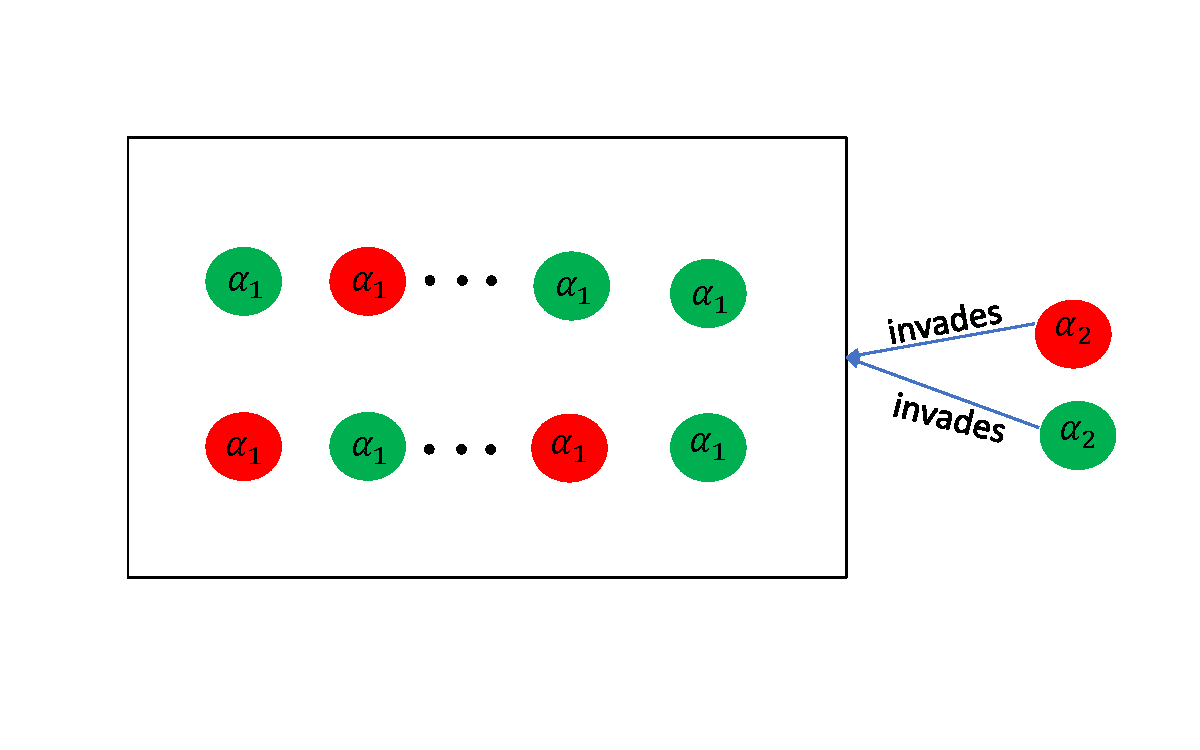
\includegraphics[width=1\textwidth]{../PRSB_figures/fig_2.pdf}
    \caption{\textbf{Evolution of cooperation under vertical, oblique, and horizontal cultural transmission.} 
    The figure shows parameter ranges for global fixation of cooperation (green), global fixation of defection (red), fixation of either cooperation or defection depending on the initial conditions, i.e. unstable polymorphism (blue), and stable polymorphism of cooperation and defection (yellow).
	In all cases the vertical transmission rate $v$ is on the x-axis.
	(\textbf{a-b})~Cost of cooperation $c$ is on the y-axis and the cost thresholds $\gamma_1$ and $\gamma_2$ (Eqs.~\ref{eq:cost_thresholds_v_threshold}) are represented by the solid and dashed lines, respectively. 
    (\textbf{c-d})~Interaction-transmission association $\alpha$ is on the y-axis and the interaction-transmission association thresholds $a_1$ and $a_2$ (Eqs.~\ref{eq:boundries_assortative_meeting_general_case}) are represented by the solid and dashed lines, respectively. 
    Horizontal transmission is biased in favor of cooperation, $T_A>T_B$, in (\textbf{a}) and (\textbf{c}), or defection, $T_A<T_B$, in (\textbf{b}) and (\textbf{d}).    
    Here, $T_A = 0.5$, and
    (\textbf{a}) $b=1.2$, , $T_B = 0.4$, $\alpha = 0.4$;
    (\textbf{b}) $b=2$, $T_B = 0.7$, $\alpha = 0.7$;
    (\textbf{c}) $b=1.2$, $T_B = 0.4$, $c=0.5$;
    (\textbf{d}) $b=2$, $T_B = 0.7$, $c=0.5$.
    }
    \label{fig:equilibria}
\end{figure}

%%% Figure: thresholds figure - only vertical

\begin{figure}[p]
  \centering       
	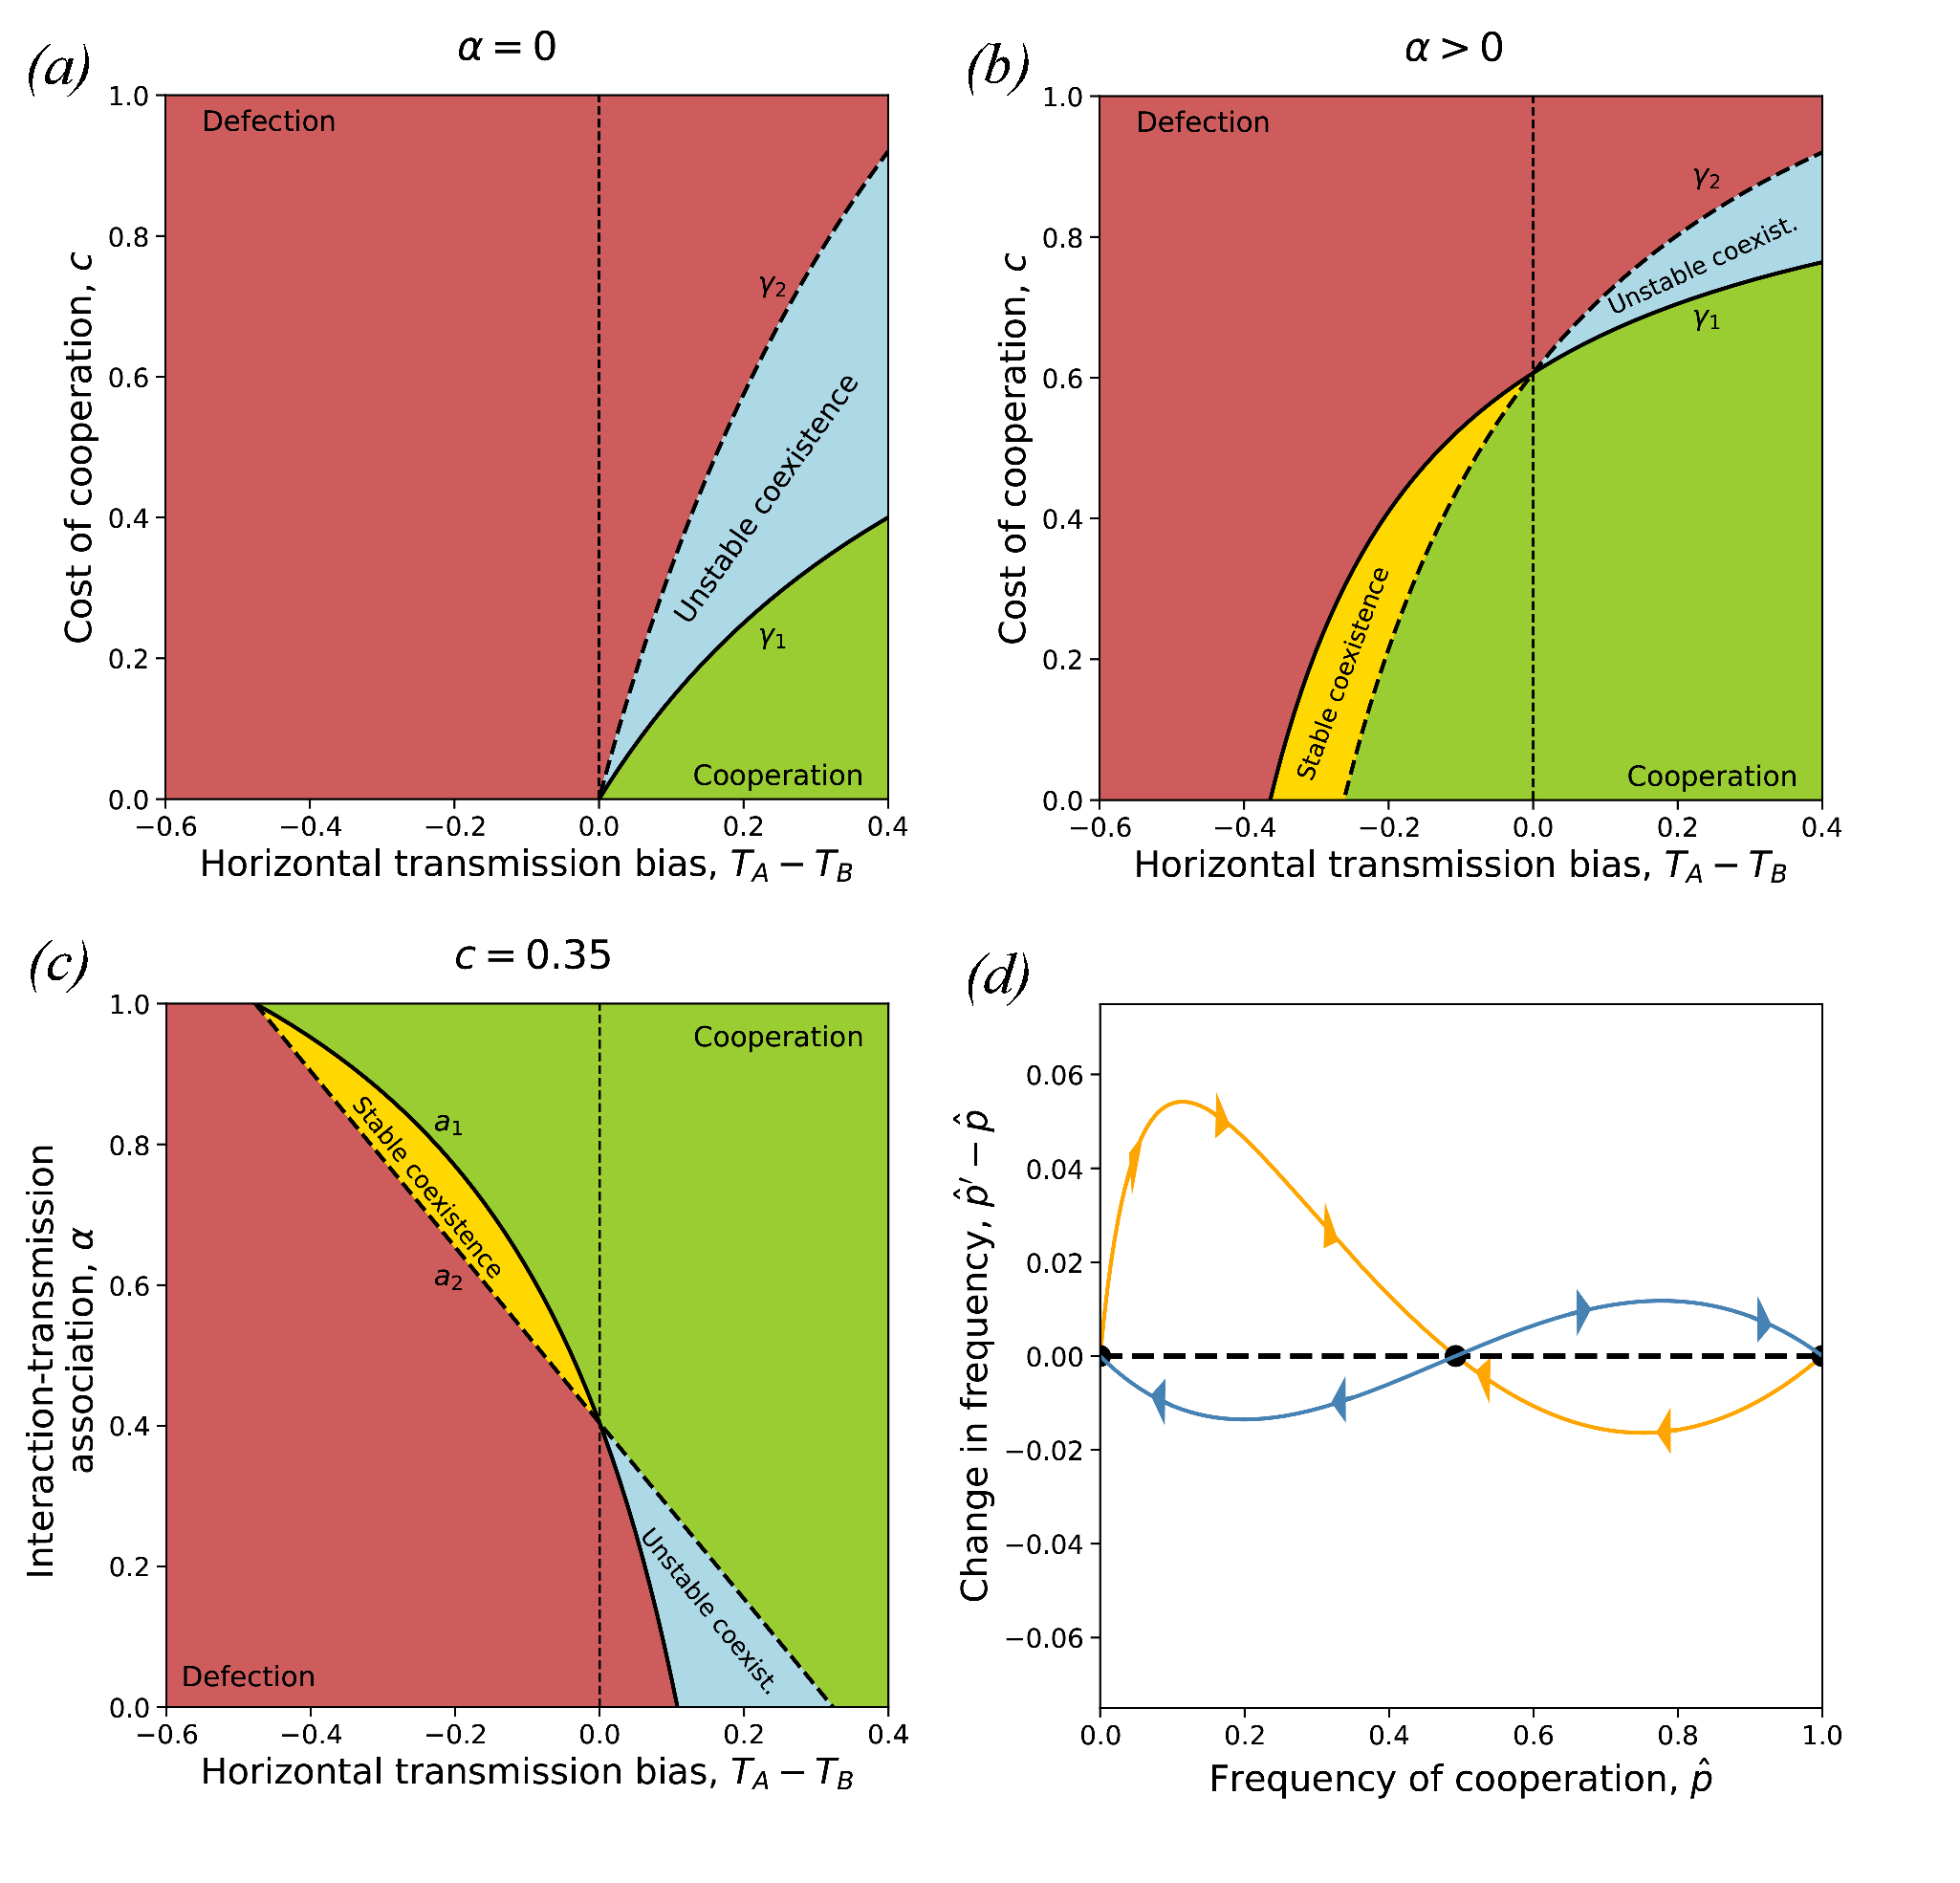
\includegraphics[width=1\textwidth]{../PRSB_figures/fig_3.pdf}
    \caption{\textbf{Evolution of cooperation under vertical and horizontal cultural transmission (v=1).} 
    The figure shows parameter ranges for global fixation of cooperation (green), global fixation of defection (red), fixation of either cooperation or defection depending on the initial conditions, i.e. unstable polymorphism (blue), and stable polymorphism of cooperation and defection (yellow).
    (\textbf{a-c})~The horizontal transmission bias ($T_A-T_B$) is on the x-axis.
    In panels \textbf{(a)} and \textbf{(b)}, the cost of cooperation $c$ is on the y-axis and the cost thresholds $\gamma_1$ and $\gamma_2$ (\autoref{eq:cost_thresholds_v_threshold}) are the solid and dashed lines, respectively. 
	In panel \textbf{(c)}, interaction-transmission association $\alpha$ is on the y-axis and the interaction-transmission association thresholds $a_1$ and $a_2$ (Eqs.~\ref{eq:boundries_assortative_meeting_general_case}) are the solid and dashed lines, respectively.
    Here, $b=1.3$, $T_A=0.4$, $v=1$, (a)~$\alpha = 0$, (b)~$\alpha = 0.7$, (c)~$c = 0.35$.    
    \textbf{(d)}~Change in frequency of cooperation among juveniles ($\hat{p}'-\hat{p}$) as a function of the frequency ($\hat{p}$), see \autoref{eq:nextgen_juveniles}.
    The orange curve shows convergence to a stable polymorphism ($T_A = 0.4$, $T_B = 0.9$, $b = 12$, $c=0.35$, $v=1$, and $\alpha = 0.45$). % todo ref eq 12
    The blue curve shows fixation of either cooperation or defection, depending on the initial frequency ($T_A = 0.5$, $T_B = 0.1$, $b = 1.3$, $c=0.904$, $v=1$, and $\alpha = 0.4$).
    Black circles show the three equilibria.
  	}
    \label{fig:equilibria_v1}
\end{figure}
\newpage

%%%%%%%%%%%%%%%%%%%%%%%%%%%%%%%%%%%%%%%%%%%%%%%%%%%%%%%
\subsection{Evolution of interaction-transmission association} 

We now focus on the evolution of interaction-transmission association under perfect vertical transmission, $v=1$, assuming that the population is initially at a stable polymorphism of the two phenotypes, cooperation $A$ and defection $B$, where the frequency of $A$ among juveniles is $\hat{p}^*$ (\autoref{eq:general_equilibrium}).
Note that for a stable polymorphism, there must be horizontal bias for defection, $T_A < T_B$, and an intermediate cost of cooperation, $\gamma_2 < c < \gamma_1$ (\autoref{eq:cost_thresholds_v_threshold}), see \autoref{fig:equilibria_v1}b.
The equilibrium population mean fitness is $\bar{w}^* = 1 + \hat{p}^*(b-c)$, which is increasing in $\hat{p}^*$, and $\hat{p}^*$ is increasing in $\alpha$ (Appendix~\ref{sec:appendixC}).
Therefore, $\bar{w}^*$ increases as $\alpha$ increases.
But can this population-level advantage lead to the evolution of $\alpha$? 

To answer this question, we add a ``modifier locus''~\citep{Feldman1972,Liberman1986general,Liberman1986modifiers,Liberman1988} that determines the value of $alpha$ but has no direct effect on fitness.
This locus has two alleles, $M$ and $m$, which induce interaction-transmission associations $\alpha_1$ and $\alpha_2$, respectively.
Suppose that the population has evolved to a stable equilibrium $\hat{p}^*$  when only allele $M$ is present.
We study the local stability of this equilibrium to invasion by the modifier allele $m$; this is called ``external stability'' \citep{Liberman1986modifiers,Altenberg2017} and obtain the following result.
\\


%%%%%%%%%%%%%%%%%%%%%%%%%%%
\begin{result}%[Reduction principle for interaction-transmission association] 
\label{result:evol_social_association}
From a stable polymorphism between cooperation and defection, a modifier allele can successfully invade the population if it decreases the interaction-transmission association $\alpha$.
\end{result}

The analysis is in Appendix~\ref{sec:appendixD}.
This reduction principle entails that successful invasions will reduce the frequency of cooperation, as well as the population mean fitness (\autoref{fig:invasion}).
Furthermore, if we a modifier allele that decreases $\alpha$ appears and invades the population from time to time, then the value of $\alpha$ will continue to decrease, further reducing the frequency of cooperation and the population mean fitness.
This evolution will proceed as long as there is a stable polymorphism, that is, as long as $a_2 < \alpha < a_1$ (Remark~\ref{remark:intermediate_association_res3}, \autoref{fig:equilibria_v1}c). 
Thus, we can expect the value of $\alpha$ to approach $a_2$, the frequency of cooperation to fall to zero, and the population mean fitness to decrease to one (\autoref{fig:invasion}).

We can do similiar analysis for the general case where $0<v<1$ as we did in Appendix~\ref{sec:appendixD}.
First we found the value of the characteristic polynomial at 1, $R(1)$ using \emph{SymPy} \citep{Meurer2017}, a Python library for symbolic mathematics.
\begin{equation} \label{eq:value_at_1}
  \begin{aligned}
  R(1) &= \frac{c v \hat{p}^*[T_Ab\hat{p}^{*2}(v\alpha_2-1)-2T_Ab\hat{p}^*v\alpha_2 + T_Ab\hat{p}^*(1+v\alpha_2)]}{b\hat{p}(b\hat{p}^*-2\hat{p}^*+2)+c\hat{p}^*(c\hat{p}^*-2)+1} \\
 & + \frac{c v \hat{p}^*[T_Ac\hat{p}^{*2}(1-v)+T_Ac\hat{p}^*(v-1)-T_A\hat{p}^*(1-c)+T_A]}{b\hat{p}(b\hat{p}^*-2\hat{p}^*+2)+c\hat{p}^*(c\hat{p}^*-2)+1} \\
  &+ \frac{c v \hat{p}^*[T_Bb\hat{p}^{*2}(1-v\alpha_2)+T_Bb\hat{p}^2(v\alpha_2-1)+T_Bc\hat{p}^{*2}(v-1)]}{b\hat{p}(b\hat{p}^*-2\hat{p}^*+2)+c\hat{p}^*(c\hat{p}^*-2)+1}\\
  &+ \frac{c v \hat{p}^*[T_Bc\hat{p}^*(1-v) + T_Bcv(1-\hat{p}^*+T_B(\hat{p}^*-1)+cv(\hat{p}^*-1))]}{b\hat{p}(b\hat{p}^*-2\hat{p}^*+2)+c\hat{p}^*(c\hat{p}^*-2)+1}
  \end{aligned}
\end{equation}
Similarly to what we did in Appendix~\ref{sec:appendixD}, we should find when $R(1)<0$. However, when adding the vertical transmission into the system the math is more complicated. 
Therefore, we will use a different technique. We know that when $\alpha_1 = \alpha_2$, $R(1)=0$. 
% DC: Yoav should I proof the statement above?
Now, let's assume that $\alpha_2 = \alpha_1 + \epsilon$. The derivative of $R(1)$ by $\epsilon$ will give us better understand about the sign of $R(1)$ when $\alpha_2<\alpha_1$.
\begin{equation} \label{eq:value_at_1_derivative}
  \frac{\partial R(1)}{\partial \epsilon} = \frac{c b  v^2 \hat{p}^*[T_A\hat{p}^{*2}-2T_A\hat{p}^* + T_A-T_B\hat{p}^{*2}+T_B\hat{p}^*]}{b\hat{p}(b\hat{p}^*-2\hat{p}^*+2)+c\hat{p}^*(c\hat{p}^*-2)+1} 
\end{equation}
We can simplify \autoref{eq:value_at_1_derivative}
\begin{equation} \label{eq:value_at_1_derivative_simplify}
  \frac{\partial R(1)}{\partial \epsilon} = \frac{c b v^2 \hat{p}^*[(T_A-T_B)\hat{p}^{*2}+(T_B-2T_A)\hat{p}^* + T_A]}{(b\hat{p}^*-c\hat{p}^*)^2+2\hat{p}^*(b-c)+1} 
\end{equation}
Since $b>c$ the denominator is always positive. The numerator is quadratic polynomial of $\hat{p}^*$ with the following roots:
\begin{equation} \label{eq:numerator_roots}
  \hat{p}^*_1 = \frac{T_A}{T_A-T_B} \hat{p}^*_2 = 1
\end{equation}
$\hat{p}^*_1 < 0$ since $T_B>T_A$ and since the quadratic polynomial has negative leading coefficient then the numerator is positive for every $\hat{p}^*_1<\hat{p}^*<1$ which is always true.
We found that derivative of $R(1)$ by $\epsilon$ is positive for every $\epsilon$. 
Therefore, $R(1)$ grows as $\epsilon$ grows, or in other words as $\alpha_2-\alpha_1$ grows.
Thus, $R(1)<0$ if and only if $\alpha_2<\alpha_1$. Therefore, different value of vertical transmission does not change the evolution of social-interaction association and invasion is possible when $\alpha_2<\alpha_1$.
% DC: can I say if and only if

%%% Figure: Invasion
\begin{figure}[h]
  \centering
  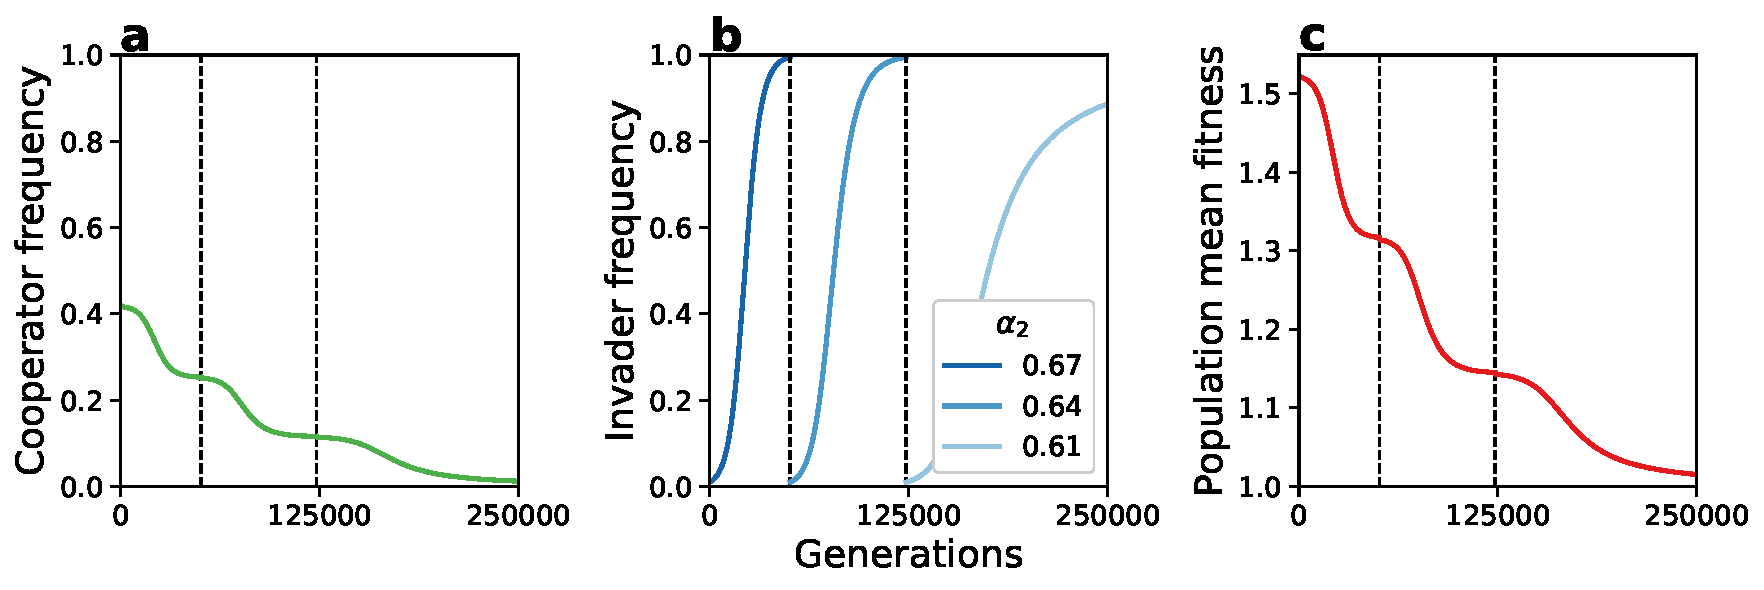
\includegraphics[width=1\textwidth]{../PRSB_figures/fig_s1.pdf}
  \caption{
  \textbf{Reduction principle for interaction-transmission association.} 
  Consecutive fixation of modifier alleles that reduce interaction-transmission association $\alpha$ in numerical simulations of evolution with two modifier alleles (Eq.~D1).
  When an invading modifier allele is established in the population (frequency > 99.95\%), a new modifier allele that reduces interaction-transmission association by 5\% is introduced (at initial frequency 0.5\%).
  \textbf{(a)}~The frequency of the cooperative phenotype $A$ over time.
  \textbf{(b)}~The frequency of the invading modifier allele $m$ over time. 
  \textbf{(c)}~The population mean fitness ($\bar{w}$) over time.
  Here, $v=1$, $c = 0.05$, $b=1.3$, $T_A=0.4<T_B=0.7$, initial interaction-transmission association $\alpha_1=0.7$, lower interaction-transmission association threshold $a_2=0.605$.  
  }
  \label{fig:invasion}
\end{figure}
\newpage
%%%%%%%%%%%%%%%%%%%%%%%%%%%%%%%%%%%%%%%%%%%%%%%%
\subsection{Population structure}
All the simulations in this section were made by Ohad Lewin-Epstein from Tel Aviv University.
Interaction-transmission association may also emerge from population structure.
Consider a  population colonizing a two-dimensional grid of size 100-by-100, where each site is inhabited by one individual, similarly to the model of \citet{lewin2020rockpaperscissors}.
Each individual is characterized by its phenotype: either cooperator, $A$, or defector, $B$.
Initially, each site in the grid is randomly colonized by either a cooperator or a defector, with equal probability.
In each generation, half of the individuals are randomly chosen to "initiate" interactions, and these
initiators interact with a random neighbor (i.e. individual in a neighboring site) in a prisoners' dilemma game (\autoref{fig:illustration}c) and a random neighbor (with replacement) for horizontal cultural transmission (\autoref{fig:illustration}b).
The expected number of each of these interactions per individual per generation is one, but the realized number of interactions can be zero, one, or even more than one, and in every interaction both individuals are affected, not just the initiator.
The effective interaction-transmission association $\alpha$ in this model is the probability that the same neighbor is picked for both interactions, or $\alpha=1/M$, where $M$ is the number of neighbors.
On an infinite grid, $M=8$ (i.e. Moore neighbourhood~\citep{moore1962machine}), but on a finite grid $M$ can be lower in neighbourhoods close to the grid border.
As before, $T_A$ and $T_B$ are the probabilities of successful horizontal transmission of phenotypes $A$ and $B$, respectively.

The order of the interactions across the grid at each generation is random.
After all interactions take place, an individual's fitness is determined by
$w = 1 + b \cdot n_b - c \cdot n_c$,
where $n_b$ is the number of interactions that individual had with cooperative neighbors,
and $n_c$ is the number of interactions in which that individual cooperated (note that the phenotype may change between consecutive interactions due to horizontal transmission).
Then, a new generation is produced, and the sites can be settled by offspring of any parent, not just the neighboring parents.
Selection is global, rather than local, in accordance with our deterministic model:
The parent is randomly drawn with probability proportional to its fitness, divided by the sum of the fitness values of all potential parents.
Offspring are assumed to have the same phenotype as their parents (i.e. $v=1$).

The outcomes of stochastic simulations with such a structured population are shown in \autoref{fig:spatial}, which demonstrates that the highest cost of cooperation $c$ that permits the evolution of cooperation agrees with the conditions derived above for our model without population structure or stochasticity.
An example of stochastic stable polymorphism is shown in \autoref{fig:spatial}c.
Changing the simulation so that selection is local (i.e. sites can only be settled by offspring of neighboring parents) had only a minor effect on the agreement with the derived conditions (\autoref{fig:spatial_local_selection}).

These comparisons between the deterministic unstructured model and the stochastic structured model show that the conditions derived for the deterministic model can be useful for predicting the dynamics under complex scenarios. 
Moreover, this structured population model demonstrates that our parameter for interaction-transmission association, $\alpha$, can represent local interactions between individuals.

\newpage

%%% Figure: Spatial model - global selection
\begin{figure}[h]
  \centering
  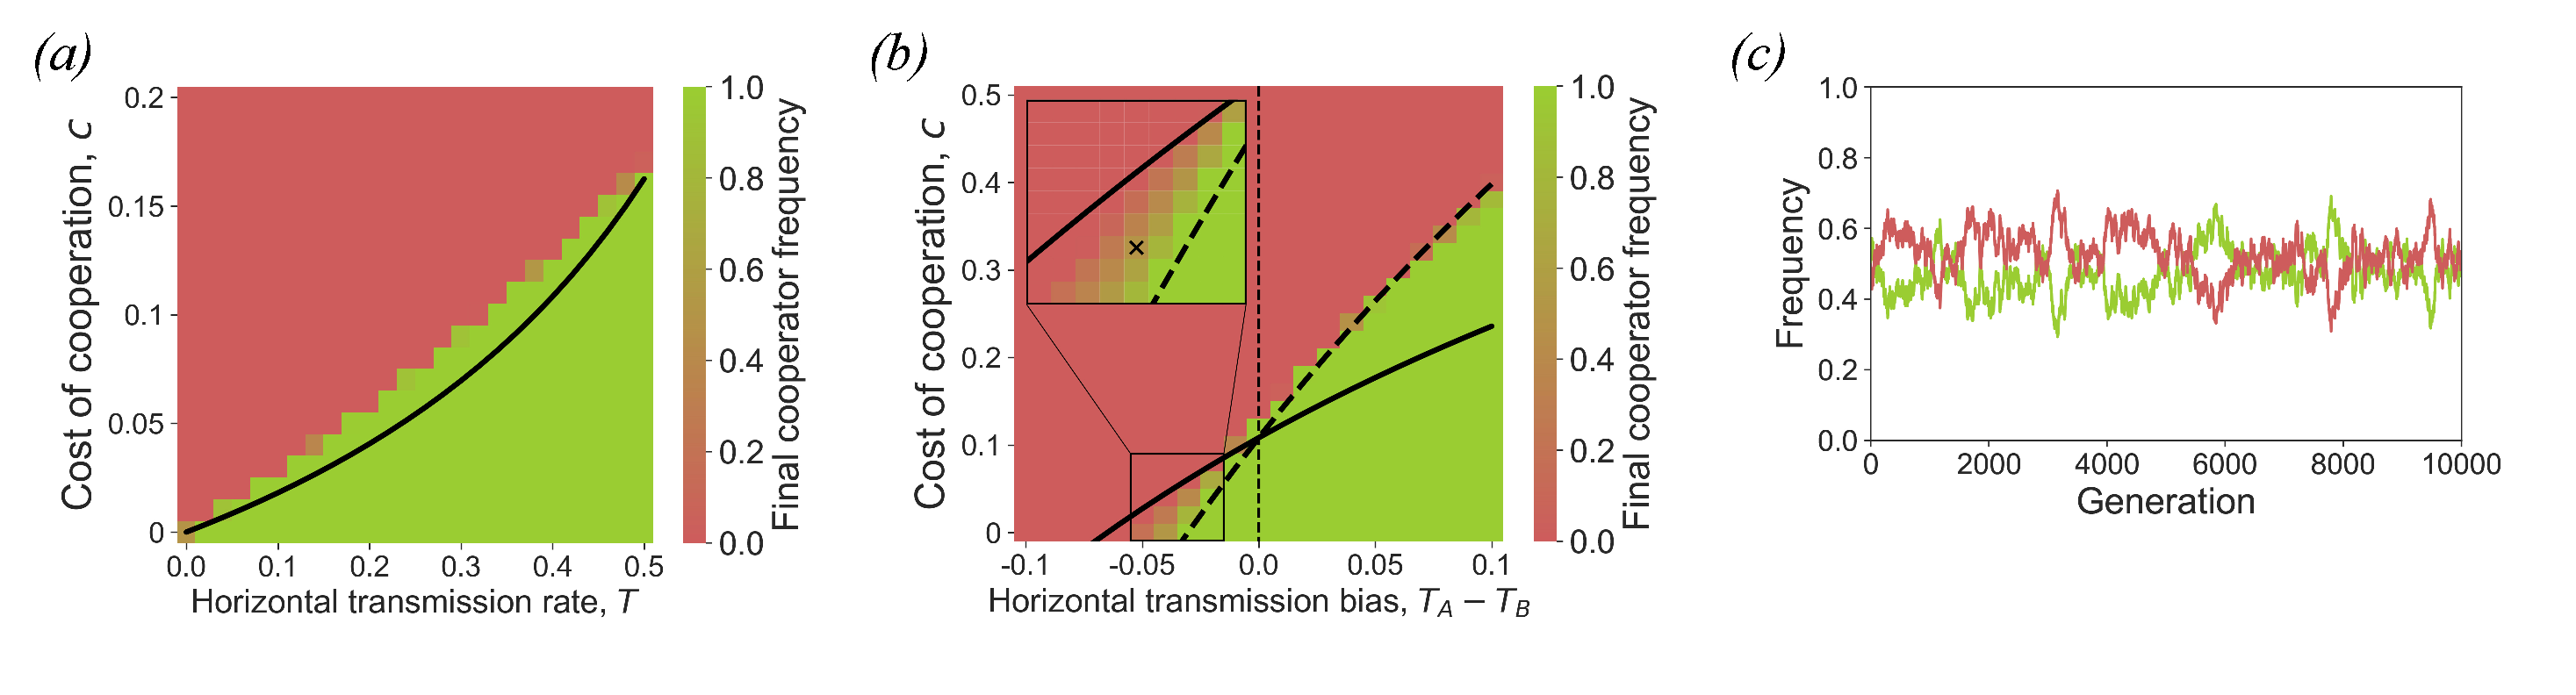
\includegraphics[width=1\textwidth]{../PRSB_figures/fig_4.pdf}
  \caption{
  \textbf{Evolution of cooperation in a structured population.}
	\textbf{(a-b)}~The expected frequency of cooperators in a structured population after 10,000 generations is shown (red for 0\%, green for 100\%) as a function of both the cost of cooperation, $c$, on the y-axis, and either the symmetric horizontal transmission rate, $T=T_A=T_B$, on the x-axis of panel~\textbf{(a)}, or the transmission bias, $T_A-T_B$, on the x-axis of panel~\textbf{(b)}.
  Black curves represent the cost thresholds for the evolution of cooperation in a well-mixed population with interaction-transmission association, where $\alpha=1/8$ in inequality~\ref{eq:equal_transmission} for  panel~\textbf{(a)} and in Eqs.~\ref{eq:cost_thresholds_v_threshold} for panel~\textbf{(b)}.
	The inset in panel~\textbf{(b)} focuses on an area of the parameter range in which neither phenotype is fixed throughout the simulation, maintaining a stochastic locally stable polymorphism~\citep{Karlin1975}.
	This stochastic polymorphism is illustrated in panel~\textbf{(c)}, which shows the frequency of cooperators (green) and defectors (red) over time for the parameter set marked by an~\textit{x} in panel~\textbf{(b)}.
  In all cases, the population evolves on a 100-by-100 grid.
  Cooperation and horizontal transmission are both local between neighbouring sites, and each site has 8 neighbours.
  Selection operates globally (see Figure S2 for results from a model with local selection).
  Simulations were stopped at generation 10,000 or if one of the phenotypes fixed. 50 simulations were executed for each parameter set.
  Benefit of cooperation, $b=1.3$; perfect vertical transmission $v=1$.
  \textbf{(a)} Symmetric horizontal transmission, $T=T_A=T_B$;
  \textbf{(b)} Horizontal transmission rate $T_A$ is fixed at $0.4$, and $T_B$ varies, $0.3<T_B<0.5$.
  \textbf{(c)} Horizontal transmission rates $T_A = 0.4 < T_B = 0.435$ and cost of cooperation $c=0.02$.
  }
  \label{fig:spatial}
\end{figure}


\newpage

%%% Figure: Spatial model - local selection
\begin{figure}[h]
  \centering
  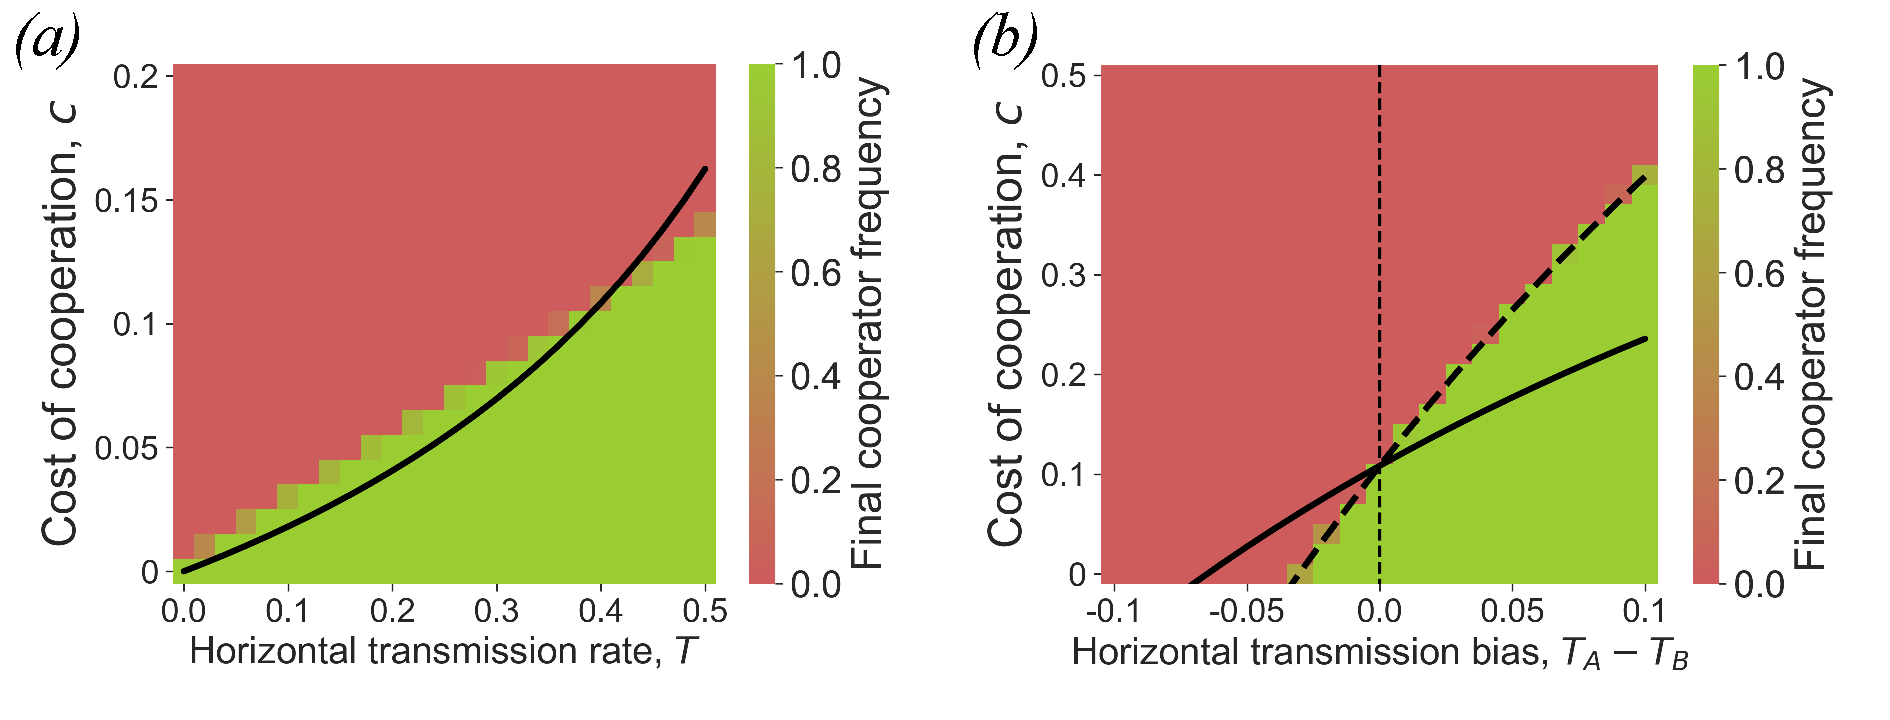
\includegraphics[width=1\textwidth]{../PRSB_figures/fig_s2.pdf}
  \caption{
  \textbf{Evolution of cooperation in a structured population with local selection.}
  The expected frequency of cooperators in a structured population after 10,000 generations is shown (red for 0\%, green for 100\%) as a function of both the cost of cooperation ($c$) on the y-axis, and the symmetric horizontal transmission rate ($T=T_A=T_B$) on the x-axis of panel~\textbf{(a)}, or the transmission bias $T_A-T_B$ on the x-axis of panel~\textbf{(b)}.
  Cooperation and horizontal transmission are both local between neighbouring sites, and each site had 8 neighbours.
  Selection operates locally (see Figure 4 for results from a model with global selection).
  The black curves represent the cost thresholds for the evolution of cooperation in a well-mixed population with interaction-transmission association, where $\alpha=1/8$ in inequality~14 for panel~\textbf{(a)} and in Eqs.~12 for panel~\textbf{(b)}.
  The population evolves on a 100-by-100 grid.
  Simulations were stopped at generation 10,000 or if one of the phenotypes fixed.
  50 simulations were executed for each parameter set.
  Here, benefit of cooperation, $b=1.3$; perfect vertical transmission $v=1$.
  \textbf{(a)} Symmetric horizontal transmission, $T=T_A=T_B$.
  \textbf{(b)} Horizontal transmission rate $T_A$ is fixed at $0.4$, and $T_B$ varies, $0.3<T_B<0.5$.
  }
  \label{fig:spatial_local_selection}
\end{figure}

%%%%%%%%%%%%%%%%%%%%%%%%%%%%%%%%%%%%%%%%%%%%%%%%%%%%%%
% Discussion
\newpage
\section{Discussion}
Under a combination of vertical, oblique, and horizontal transmission with payoffs in the form of a prisoner's dilemma game, cooperation or defection can either fix or coexist, depending on the relationship between the cost and benefit of cooperation, the horizontal transmission bias, and the association between social interaction and horizontal transmission (Result~\ref{result:vert_obli_hori}, Figures~\ref{fig:equilibria} and~\ref{fig:equilibria_v1}).
Importantly, cooperation can increase when initially rare (i.e. invade a population of defectors) if and only if, rewriting inequality~\ref{eq:unequal_transmission_from_rarity_general_case},
$
c \cdot v (1-T_B) < b \cdot v \alpha T_A + (T_A - T_B) \;,
$
namely, the effective cost of cooperation (left-hand side) is smaller then the effective benefit plus the horizontal transmission bias (right-hand side).
This condition cannot be formulated in the form of Hamilton's rule, $c<b \cdot r$, due to the effect of biased horizontal transmission, represented by $(T_A-T_B)$.
Remarkably, a polymorphism of cooperation and defection can be stable if horizontal transmission is biased in favor of defection ($T_A<T_B$) and both $c$ and $\alpha$ are intermediate (yellow areas in Figures~\ref{fig:equilibria} and~\ref{fig:equilibria_v1}).

We find that stronger interaction-transmission association $\alpha$ leads to evolution of higher frequency of cooperation and increased population mean fitness.
Nevertheless, when cooperation and defection coexist, $\alpha$ is expected to be reduced by natural selection, leading to extinction of cooperation and decreased population mean fitness (Result~\ref{result:evol_social_association}, \autoref{fig:invasion}).
With $\alpha=0$, the benefit of cooperation cannot facilitate its evolution; it can only succeed if horizontal transmission is biased in its favor. 

Indeed, in our model, horizontal transmission plays a major role in the evolution of cooperation: increasing the transmission of cooperation, $T_A$, or decreasing the transmission of defection, $T_B$, facilitates the evolution of cooperation. 
However, the effect of oblique transmission is more complicated.
When there is horizontal transmission bias in favor of cooperation, $T_A>T_B$, increasing the rate of oblique transmission, $1-v$, will facilitate the evolution of cooperation.
In contrast, when the bias is in favor of defection, $T_A<T_B$, higher rates of vertical transmission, $v$, are advantageous for cooperation, and the rate of vertical transmission must be high enough ($v>\hat v$) for cooperation to fix in the population.

Our deterministic model provides a good approximation to outcomes of simulations of a complex stochastic model with population structure in which individuals can only interact with and transmit to their neighbors.
In these structured populations interaction-transmission association arises due to both social interactions and horizontal cultural transmission being local (\autoref{fig:spatial} and \autoref{fig:spatial_local_selection}).
We did not find any significant difference between local and global selection. %DC: can we disucss why there is not difference?


\citet{feldman1985gene} studied the dynamics of an altruistic phenotype with vertical cultural transmission and a gene that modifies the transmission of the phenotype. Their results are very sensitive to this genetic modification: without it, the conditions for invasion of the altruistic phenotype reduce to Hamilton's rule.
Further work is needed to incorporate such genetic modification of cultural transmission into our model. %DC: let's discuss it maybe we can do it.
\citet{woodcock2006significance} stressed the significance of non-vertical transmission for the evolution of cooperation and
carried out simulations with prisoner's dilemma payoffs but without horizontal transmission or interaction-transmission association ($\alpha=0$).
Nevertheless, his results demonstrated that it is possible to sustain altruistic behavior via cultural transmission for a substantial length of time.
He further hypothesized that horizontal transmission can play an important role in the evolution of cooperation, and our results provide strong evidence for this hypothesis. 

To understand the role of horizontal transmission, we first review the role of \emph{assortment}.
\citet{Eshel1982} showed that altruism can evolve when the tendency for \emph{assortative meeting}, i.e. for individuals to interact with others of their own phenotype, is strong enough.
\citet{Fletcher2009assortment}  further argued that a general explanation for the evolution of altruism is given by \emph{assortment}: the correlation between individuals that carry an altruistic trait and the amount of altruistic behavior in their interaction group (see also \citet{Bijma2010assortment}).
They suggested that to explain the evolution of altruism, we should seek mechanisms that generate  assortment, such as population structure, repeated interactions, and individual recognition.
Our results highlight another mechanism for generating assortment: an association between social interactions and horizontal transmission that creates a correlation between one's partner for interaction and the partner for transmission.
This mechanism does not require repeated interactions, population structure, or individual recognition.
We show that high levels of such interaction-transmission association greatly increase the potential for evolution of cooperation.
With enough interaction-transmission association, cooperation can increase in frequency when initially rare even when there is horizontal transmission bias against it ($T_A<T_B$).

How does non-vertical transmission generate assortment? 
\citet{lewin2017microbes} and \citet{lewin2020rockpaperscissors} 
suggested that microbes that induce their hosts to act altruistically can be favored by selection, which may help to explain the evolution of cooperation. 
Indeed, it has been shown that microbes can mediate behavioral changes in their  hosts~\citep{dobson1988population,poulin2010parasite}. 
Therefore, natural selection on microbes may favor manipulation of the host so that it cooperates with others.
From the kin selection point-of-view, if microbes can be transmitted \emph{horizontally} from one host to another during host interactions, then following horizontal transmission the recipient host will carry microbes that are closely related to those of the donor host, 
even when the two hosts are (genetically) unrelated. 
From the assortment point-of-view,
infection by behavior-determining microbes during interactions effectively generates assortment because a recipient of help may be infected by a behavior-determining microbe and consequently become a helper.
Cultural horizontal transmission can similarly generate assortment between cooperators and enhance the benefit of cooperation if cultural transmission and helping interactions occur between the same individuals, i.e. when there is interaction-transmission association, so that the recipient of help may also be the recipient of the cultural trait for cooperation. 
Thus, with horizontal transmission, ``assortment between focal cooperative players and cooperative acts in their interaction
environment''~\citep{Fletcher2009assortment} is generated not because the helper is likely to be helped, but rather because the helped is likely to become a helper.

Another mechanism that was suggested by \citet{traxler2011social} showed that \emph{conditional cooperation} based on norm-dependent relational utilities, i.e. individual will only cooperate if it knows that others will cooperate too, can sustain cooperation in a community – provided that cooperation is already at a high level.
Unlike \emph{conditional cooperation}, interaction-transmission association can sustain cooperation in community even if cooperation is initially rare. 
\citet{morsky2020false} suggested that false beliefs on the frequencies of the cooperator can affect the individual decision whether to cooperate or not. If the individual over estimate the number of cooperators it will be more likely to cooperate. This flase belief can help sustain cooperation even if cooperartion is initially rare. 
% DC: Let's discuss this paragraph - is it good? 



\newpage
%%%%%%%%%%%%%%%%%%%%%%%%%%%%%%%%%%%%%%%%%%%%%%%%%%%%%%
% Bibliography
\begingroup
 \bibliographystyle{unsrtnat}
 \linespread{1}\selectfont
 \setlength{\bibsep}{2pt}
 \bibliography{bib}
\endgroup


%%%%%%%%%%%%%%%%%%%%%%%%%%%%%%%%%%%%%%%%%%%%%%%%%%%%%%



%%%%%%%%%%%%%%%%%%%%%%%%%%%%%%%%%%
\newpage
\beginsupplement % https://support.authorea.com/en-us/article/how-to-create-an-appendix-section-or-supplementary-information-1g25i5a/

%%%%%%%%%%%%%%%%%%%%%%%%%%%%%%%%%%%%%%%%%%%%%%%%%%%%%%
% Appendices
\begin{appendices}
\linespread{1.25}
\renewcommand{\theequation}{\thesection\arabic{equation}}
\counterwithin*{equation}{section}


%%%%%%%%%%%%%%%%%%%%%%%%%%%%%%%%%%%%%%%%%%%%%%%%%%%%
\section{Local stability criterion} \label{sec:appendixA}


Let $f(p)=\lambda \cdot (p'-p)$, where $\lambda>0$, and $0$ and $1$ are equilibria, that is, $f(0)=0$ and $f(1)=0$.

Set $p>p^*=0$.
Using a linear approximation for $f(p)$ near $0$, we have
\begin{equation}
p' < p \Leftrightarrow 
f(p)/p < 0 \Leftrightarrow 
\frac{f'(0) \cdot p + O(p^2)}{p} < 0 \Leftrightarrow 
f'(0) + O(p) < 0 \;.
\end{equation}
Therefore, by definition of big-O notation, if $f'(0)<0$ then there exists $\epsilon>0$ such that for any local perturbation $0<p<\epsilon$, it is guaranteed that $0<p'<p$; that is, $p'$ is closer to zero than $p$.

Set $p<p^*=1$
Using a linear approximation for $f(p)$ near $1$, we have
\begin{equation}
1-p' < 1-p  \Leftrightarrow 
-\frac{f(p)}{1-p} < 0 \Leftrightarrow 
\frac{f'(1)(p-1) + O\big((p-1)^2\big)}{p-1} < 0 \Leftrightarrow 
f'(1) - O(1-p) < 0 \;.
\end{equation}
Therefore, if $f'(1)<0$ then there exists $\epsilon>0$ such that for any $1-\epsilon<1-p<1$ we have $1-p'<1-p$; that is, $p'$ is closer to one than $p$.


%%%%%%%%%%%%%%%%%%%%%%%%%%%%%%%%%%%%%%%%%%%%%%%%%%%%%
\newpage
\section{Equilibria and stability} \label{sec:appendixB}

Let $f(\hat{p}) = \bar{w}(\hat{p}' - \hat{p})$.
Then, using \emph{SymPy} \citep{Meurer2017}, a Python library for symbolic mathematics, this simplifies to
\begin{equation} \label{eq:general_case_polynomial}
\begin{aligned}
  f(\hat{p}) &= \bar{w}(\hat{p}'-\hat{p}) =
  \beta_1 \hat{p}^3 + \beta_2 \hat{p}^2 + \beta_3 \hat{p} \;,
\end{aligned}
\end{equation}
where 
\begin{equation} \label{eq:polynomial_coefficients}
\begin{aligned}
  \beta_1 &= \big[c(1-v) - b (1-\alpha v)\big] (T_A-T_B) \;, \\
  \beta_2 &= -\beta_1 -\beta_3 \;, \\
  \beta_3 &= \alpha bvT_A - cv(1-T_B) + (T_A-T_B) \;.
\end{aligned}
\end{equation}

If $T=T_A=T_B$ then $\beta_1=0$ and $\beta_3=-\beta_2=\alpha b vT -cv(1-T)$, and $f(\hat{p})$ becomes a quadratic polynomial,
\begin{equation} \label{eq:equal_horizontal_transmission}
  f(\hat{p}) = \hat{p}(1-\hat{p})\big[\alpha bvT - cv(1-T)\big] \;.
\end{equation}
Clearly the only two equilibria are the fixations $\hat{p} =  0$ and $\hat{p} = 1$, which are are locally stable if $f'(\hat{p})<0$ near the equilibrium (see Appendix~\ref{sec:appendixA}), where
$f'(\hat{p})=(1-2\hat{p})\big[\alpha bvT - cv(1-T)\big]$, so that
\begin{equation} \label{eq:derivative_of_phattag-phat}
\begin{aligned}
	f'(0) &=	\alpha bvT - cv(1-T) \;, \\
	f'(1) &=	-\alpha bvT + cv(1-T) \;.
\end{aligned}
\end{equation}

In the general case where $T_A \neq T_B$, the coefficient $\beta_1$ is not necessarily zero, and $f(\hat{p})$ is a cubic polynomial.
Therefore, three equilibria may exist, two of which are
$\hat{p} = 0 $ and $\hat{p} = 1$, and the third is
\begin{equation} \label{eq:general_equilibrium_appendix}
  \hat{p}^* =  
  \frac{\beta_3}{\beta_1} =
  \frac{\alpha bvT_A - cv(1-T_B) + (T_A-T_B)}{\big[c(1-v) - b (1-\alpha v)\big] (T_A-T_B)} \;.
\end{equation}

Note that the sign of the cubic (Eq.\ \ref{eq:general_case_polynomial}) at positive (negative) infinity is equal (opposite) to the sign of $\beta_1$. 
If $T_A>T_B$, then 
\begin{equation} \label{eq:beta1}
   \beta_1 < [c(1-\alpha v) - b(1-\alpha v)] (T_A-T_B) 
   = (1-\alpha v)(c-b)(T_A-T_B) < 0 \;,
 \end{equation}
since $c<b$ and $\alpha v < 1$. Hence the signs of the cubic at positive and negative infinity are negative and positive, respectively.
First, if $\beta_3<\beta_1$ then 
$1<\hat{p}^*$. Also, $f'(0)<0$ and $f'(1)>0$; that is, fixation of the defector phenotype $B$ is the only locally stable feasible equilibrium.
Second, if $\beta_1<\beta_3<0$ then 
$0<\hat{p}^*<1$ and therefore $f'(0)<0$ and $f'(1)<0$ so that both fixations are locally stable and $\hat{p}^*$ separates the domains of attraction.
Third, if $0<\beta_3$ then 
$\hat{p}^*<0$ and therefore $f'(0)>0$ and $f'(1)<0$; that is, fixation of the cooperator phenotype $A$ is the only locally stable legitimate equilibrium.

Similarly, if $T_A<T_B$, then
\begin{equation} \label{eq:beta1_rev}
   \beta_1 > [c(1-\alpha v) - b(1-\alpha v)] (T_A-T_B) 
   = (1-\alpha v)(c-b)(T_A-T_B) > 0 \;,
 \end{equation}
since $c<b$ and $\alpha v < 1$, and the signs of the cubic at positive and negative infinity are positive and negative, respectively. 
First, if $\beta_3<0$ then $\hat{p}^*<0$ and therefore $f'(0)<0$ and $f'(1)>0$; that is, fixation of the defector phenotype $A$ is the only locally stable legitimate equilibrium.
Second, if $0<\beta_3<\beta_1$ then $0<\hat{p}^*<1$ and therefore $f'(0)>0$ and $f'(1)>0$; that is, both fixations are locally unstable and $\hat{p}^*$ is a stable polymorphic equilibrium.
Third, if $\beta_1<\beta_3$ then $\hat{p}^*>1$ and therefore $f'(0)>0$ and $f'(1)<0$, and fixation of the cooperator phenotype $A$ is the only locally stable feasible equilibrium.

This analysis can be summarized as follows:
% in beta
\begin{enumerate}
\item \emph{Fixation of cooperation}: 
	if \emph{(i)} $T=T_A=T_B$ and $c < b\cdot \frac{\alpha T}{1-T}$; or
	if \emph{(ii)} $T_A>T_B$ and $0<\beta_3$; or 
	if \emph{(iii)} $T_A<T_B$ and $\beta_1<\beta_3$.
\item \emph{Fixation of the defection}: 
	if \emph{(iv)}  $T=T_A=T_B$ and $c > b\cdot \frac{\alpha T}{1-T}$; or 
	if \emph{(v)} $T_A>T_B$ and $\beta_3<\beta_1<0$; or 
	if \emph{(vi)} $T_A<T_B$ and $\beta_3<0$.
\item \emph{polymorphism of both phenotypes at $\hat{p}^*$}: 
	if \emph{(vii)} $T_A < T_B$ and $0<\beta_3<\beta_1$.
\item \emph{Fixation of either phenotype depending on initial frequency}:
	if \emph{(viii)}  $T_A>T_B$ and $\beta_1<\beta_3<0$.
\end{enumerate}

We now proceed to use the cost thresholds, $\gamma_1$ and $\gamma_2$, and the vertical transmission threshold, $\hat v$ (\autoref{eq:cost_thresholds_v_threshold}).
First, assume $T_A<T_B$.
$\beta_3<0$ requires $\gamma_1<c$.
For $\beta_3<\beta_1$ we need $c\big[v(1-T_B) + (1-v)(T_A-T_B)\big] > bv\alpha T_B + (1+b)(T_A-T_B)$.
Note that the expression in the square brackets is positive if and only if $v > \hat v$.
Thus, for $\beta_3<\beta_1$ we need $v > \hat v$ and $\gamma_2 < c$ or $v < \hat v$ and $c < \gamma_2$,
and for $0<\beta_3<\beta_1$ we need $v > \hat v$ and $\gamma_2 < c < \gamma_1$, or $v < \hat v$ and $c < \min(\gamma_1, \gamma_2)$. For $\beta_1<\beta_3$ we need $v > \hat v$ and $c<\gamma_2$ or $v < \hat v$ and $\gamma_2<c$.
However, some of these conditions cannot be met, since $v < \hat v$ implies $c<1<\gamma_2$.

Second, assume $T_A>T_B$.
$\beta_3>0$ requires $\gamma_1 > c$. 
For $\beta_1<\beta_3$ we need $c\big[v(1-T_B) + (1-v)(T_A-T_B)\big] < bv\alpha T_B + (1+b)(T_A-T_B)$.
Thus for $\beta_1<\beta_3$ we need $v > \hat v$ and $c < \gamma_2 $ or $v < \hat v$ and $c > \gamma_2$.
But $\hat{v}<0$ when $T_A > T_B$, and therefore we have $\beta_1<\beta_3$ if $c < \gamma_2$. Similarly, we have $\beta_3<\beta_1$ if $c > \hat{\gamma_2}$.

This analysis is summarized in Result~\ref{result:vert_obli_hori}.

%%%%%%%%%%%%%%%%%%%%%%%%%%%%%%%%%%%%%%%%%%%%%%%%%%%%%
\newpage
\section{Effect of interaction-transmission association on mean fitness} \label{sec:appendixC}

To determine the effect of increasing $\alpha$ on the stable population mean fitness, $\bar{w}^*=1+(b-c)\hat{p}^*$, we must analyze its effect on $\hat{p}^*$, 
\begin{equation} \label{eq:mean_fitness_stable_polymorphism_derivative}
  \frac{\partial \hat{p}^*}{\partial \alpha} 
%  =\frac{-b^2T_A (1-\alpha) (T_A-T_B) + b(T_A-T_B)(c(1-T_B) - b \alpha T_A - (T_A-T_B))}{b^2 (1-\alpha)^2 (T_A-T_B)^2} 
%  = \frac{b^2T_A(T_B-T_A)-bc(1-T_B)(T_B-T_A) - b(T_B-T_A)^2}{b^2 (1-\alpha)^2 (T_A-T_B)^2} \;.
  = \frac{b T_A - c(1-T_B) + (T_A-T_B)}{b (1-\alpha)^2 (T_B-T_A)} \;.
\end{equation} 
Note that stable polymorphism implies $c<\gamma_1$, and because $\alpha<1$, we have
\begin{equation}
c < \gamma_1 = \frac{b \alpha T_A + (T_A-T_B)}{1-T_B} < \frac{b T_A + (T_A-T_B)}{1-T_B}.
\end{equation} 
Therefore, the numerator in \autoref{eq:mean_fitness_stable_polymorphism_derivative} is positive.
Since $T_A<T_B$, the denominator in \autoref{eq:mean_fitness_stable_polymorphism_derivative} is also positive, and hence the derivative $\partial \hat{p}^* / \partial \alpha$ is positive.
Thus, the population mean fitness increases as interaction-transmission association $\alpha$ increases.



%%%%%%%%%%%%%%%%%%%%%%%%%%%%%%%%%%%%%%%%%%%%%%%%%%%%%
\newpage
\section{Reduction principle} \label{sec:appendixD}

We assume here that $v=1$, i.e. no oblique transmission, and therefore $\hat{p}=\dot{p}$.
Denote the frequencies of the pheno-genotypes $AM$, $BM$, $Am$, and $Bm$ by $\vec{\dot{p}}= (\dot{p}_1$, $\dot{p}_2$, $\dot{p}_3$, $\dot{p}_4)$. 
The frequencies of the pheno-genotypes in the next generation are defined by the recursion system, 
\begin{equation} \label{eq:next_gen_p_1}
  \begin{aligned}
	% p1
  \bar{w}\dot{p}_1' = 
  & \dot{p}_1 x (1+b-c)(1 - (1-\alpha_1)(1-x)T_B) \;+ \\
  & \dot{p}_1(1-x)(1-c)(1-\alpha_1T_B x - T_B(1-x)) \;+ \\
  & \dot{p}_2 x (1+b)T_A(x + \alpha_1(1-x)) \;+ \\
  & \dot{p}_2(1-x)x(1-\alpha_1)T_A \;,
\\
	% p2
  \bar{w}\dot{p}_2' = 
  & \dot{p}_1 x (1+b-c)(1-\alpha_1)(1-x)T_B \;+ \\
  & \dot{p}_1(1-x)(1-c)(\alpha_1 T_B + (1-\alpha_1)(1-x)T_B) \;+ \\
  & \dot{p}_2 x (1+b)(1-\alpha_1 T_A(1-x) - T_A x) \;+ \\
& \dot{p}_2(1-x)(1 - (1-\alpha_1) x T_A) \;, 
\\
	% p3
  \bar{w}\dot{p}_3' =
  & \dot{p}_3 x (1+b-c)(1 - (1-\alpha_2)(1-x)T_B) \;+ \\
  & \dot{p}_3(1-x)(1-c)(1-\alpha_2 T_B x - T_B(1-x)) \;+ \\
  & \dot{p}_4 x (1+b)T_A(x + \alpha_2 (1-x)) \;+ \\
  & \dot{p}_4(1-x) x (1-\alpha_2)T_A \;, 
\\
	% p4
  \bar{w}\dot{p}_4' =
  & \dot{p}_3 x (1+b-c)(1-\alpha_2)(1-x)T_B \;+ \\
  & \dot{p}_3(1-x)(1-c)(\alpha_2 T_B + (1-\alpha_2)(1-x)T_B) \;+ \\
  & \dot{p}_4 x (1+b)(1-\alpha_2T_A(1-x)-T_A x ) \;+ \\
  & \dot{p}_4(1-x)(1 - (1-\alpha_2) x T_A) \;,
  \end{aligned}
\end{equation}
%which we can write as 
%\begin{equation}
%\bar{w} \vec{\dot{p}} = F(\vec{\dot{p}}),
%\end{equation}
where $x=\dot{p}_1+\dot{p}_3$ is the total frequency of the cooperative phenotype $A$, and $\bar{w} = 1 + (b-c) x$ is the population mean fitness.% and $\vec{\dot{p}} = (\dot{p}_1,\dot{p}_2,\dot{p}_3,\dot{p}_4)$.

The equilibrium where only allele $M$ is present is  $\vec{\dot{p}^*} = (\dot{p}^*, 1-\dot{p}^*, 0, 0)$, where
\begin{equation} \label{eq:p_tilde_star_alpha_1}
\dot{p}^*=
\frac{c(1-T_B) - b \alpha_1 T_A - (T_A - T_B)}{b(1-\alpha_1)(T_A-T_B)} \;,
\end{equation}
setting $\alpha=\alpha_1$ and $v=1$ in \autoref{eq:general_equilibrium}.
When $v=1$, $\dot p^*$ is a feasible polymorphism ($0 < \dot{p}^* < 1$) if $T_A<T_B$ and $\gamma_2<c<\gamma_1$ (Result~\ref{result:vert_obli_hori}).

The local stability of $\vec{\dot{p}^*}$ to the introduction of allele $m$ is determined by the linear approximation $\cl^*$ of the transformation in \autoref{eq:next_gen_p_1} near $\vec{\dot{p}^*}$ (i.e. the Jacobian of the transformation at the equilibrium).
$\cl^*$ is known to have a block structure, with the diagonal blocks occupied by the matrices $\cl^*_{in}$ and $\cl^*_{ex}$ \citep{Liberman1986modifiers,Altenberg2017} .
The latter is the external stability matrix: the linear approximation to the transformation near $\vec{\dot{p}^*}$ involving only the pheno-genotypes $Am$ and $Bm$, derived from \autoref{eq:next_gen_p_1}, with $\bar{w}^*=1+(b-c)\dot{p}^*$ as the stable population mean fitness,
\begin{equation} \label{eq:external_stability_matrix}
\begin{aligned}
&\cl^*_{ex} = 
 \frac{1}{\bar{w}^*} \begin{bmatrix}
	 l_{1 1} &
	 l_{1 2} \\
	 l_{2 1} &
	 l_{2 2} 
\end{bmatrix} = 
\frac{1}{\bar{w}^*} \begin{bmatrix}
\frac{\partial\bar{w}\dot{p}_3'}{\partial \dot{p}_3}(\vec{\dot{p}}^*) &
\frac{\partial\bar{w}\dot{p}_3'}{\partial \dot{p}_4}(\vec{\dot{p}}^*) \\
\frac{\partial\bar{w}\dot{p}_4'}{\partial \dot{p}_3}(\vec{\dot{p}}^*) &
\frac{\partial\bar{w}\dot{p}_4'}{\partial \dot{p}_4}(\vec{\dot{p}}^*) 
\end{bmatrix} \;= \\
& \frac{1}{\bar{w}^*} \begin{bmatrix}
		(1+b \dot{p}^* -c)(1-T_B(1-\dot{p}^*)) + b \dot{p}^* \alpha_2 T_B (1-\dot{p}^*) & 
		(1+b \dot{p}^*) T_A \dot{p}^* + b \dot{p}^* \alpha_2 T_A(1-\dot{p}^*) \\
		(1+b \dot{p}^* - c) T_B(1-\dot{p}^*) - b \dot{p}^* \alpha_2 T_B (1-\dot{p}^*) &
		(1+b \dot{p}^*) (1-T_A \dot{p}^*) - b \dot{p}^* \alpha_2 T_A (1-\dot{p}^*) \\
  	\end{bmatrix} \;.
\end{aligned}
\end{equation}

Because we assume that $\vec{\dot{p}^*}$ is internally stable (i.e. locally stable to small perturbations in the frequencies of $AM$ and $BM$), the stability of 
$\vec{\dot{p}^*}$ is determined by the eigenvalues of the external stability matrix $\cl^*_{ex}$.
This is a positive matrix, and due to the Perron-Frobenius theorem, the leading eigenvalue of $\cl^*_{ex}$ is real and positive.
Thus, if the leading eigenvalue is less (greater) than one, then the equilibrium $\vec{\dot{p}^*}$ is externally stable (unstable) and allele $m$ cannot (can) invade the population of allele $M$. 
The eigenvalues of $\cl^*_{ex}$ are the roots of the characteristic polynomial, $R(\lambda)$,
%\begin{equation}\label{char_poly}
%R(\lambda) = 
%\lambda^2 -\lambda \frac{(X+Q)}{\bar{w^*}} + \frac{XQ - YZ}{\bar{w^*}^2} \;,
%\end{equation}
%where $X$, $Y$, $Z$, and $Q$ are defined in \autoref{eq:external_stability_matrix}.
which is a quadratic with a positive leading coefficient. Therefore, $\lim_{\lambda \to \pm \infty} R(\lambda) = \infty$, and the leading eigenvalue is less than one (implying stability) if and only if $R(1)>0$ and $R'(1)>0$.
Thus, a sufficient condition for external instability of $\vec{\dot{p}^*}$ is $R(1) < 0$.
%\begin{equation} \label{eq:R1_negative}
%\begin{aligned}
%R(1) < 0 \Leftrightarrow 
%1 - \frac{(X+Q)}{\bar{w^*}} + \frac{XQ - YZ}{\bar{w^*}^2} < 0 \Leftrightarrow 
%\bar{w^*}^2 - \bar{w^*} (X+Q) + XQ - YZ < 0 \;.
%\end{aligned}
%\end{equation}

$R(\lambda)$ is defined as a determinant, $R(\lambda)=\det(\cl^*_{ex} - \lambda \ci)$, where $\ci$ is the 2-by-2 identity matrix. 
Since multiplication by a positive factor doesn't change the sign, and using the properties of the determinant,  we have
\begin{equation} \label{eq:signR1}
\begin{aligned}
\sign R(1) =
& \sign\det(\cl^*_{ex} - \ci) =
  \sign (\bar{w}^*)^2 \det(\cl^*_{ex} - \ci) = \\
& \sign \det(\bar{w}^*\cl^*_{ex} - \bar{w}^* \ci) =
  \sign \det\begin{bmatrix} l_{1 1} - \bar{w}^* & l_{1 2} \\ l_{2 1} & l_{2 2} - \bar{w}^* \end{bmatrix} \;,
\end{aligned}
\end{equation}
where $l_{i j}$ are defined in \autoref{eq:external_stability_matrix}.
Adding the second row in \autoref{eq:signR1} to the first row,  which does not change the determinant, and substituting $\bar{w}^*=1+(b-c)\dot{p}^*$, we get
\begin{equation} 
\begin{aligned}
\sign R(1) =
& \sign\det\begin{bmatrix}
	 -c(1-\dot{p}^*) &&
	 c \dot{p}^* \\
	 (1-\dot{p}^*)\big[(1+b\dot{p}^*-c)T_B - b \alpha_2 T_B \dot{p}^* \big] &&
	 \dot{p}^*\big[-(1+b\dot{p}^*)T_A - b \alpha_2 T_A (1-\dot{p}^*) + c\big]
\end{bmatrix} = \\
& \sign \Bigg[c \dot{p}^* (1-\dot{p}^*) \cdot \det\begin{bmatrix}
	 -1 &&
	 1 \\
	 (1+b\dot{p}^*-c)T_B - b \alpha_2 T_B \dot{p}^* &&
	 -(1+b\dot{p}^*)T_A - b \alpha_2 T_A (1-\dot{p}^*) + c
\end{bmatrix}\Bigg] = \\
& \sign\det\begin{bmatrix}
	 -1 &&
	 1 \\
	 (1+b\dot{p}^*-c)T_B - b \alpha_2 T_B \dot{p}^* &&
	 -(1+b\dot{p}^*)T_A - b \alpha_2 T_A (1-\dot{p}^*) + c
\end{bmatrix} \;,
\end{aligned}
\end{equation}
since $c>0$, $0<\dot{p}^*<1$.
That is, 
\begin{equation}
\begin{aligned}
\sign R(1) = 
&\sign\Big[
(1+b\dot{p}^*)T_A + b\alpha_2 T_A (1-\dot{p}^*) - c - 
(1+b\dot{p}^*-c)T_B + b\dot{p}^* \alpha_2 T_B \Big]
= \\
&\sign\Big[(1+b(1-\alpha_2)\dot{p}^*)(T_A-T_B) + b\alpha_2 T_A - c (1-T_B) \Big]\;.
\end{aligned}
\end{equation}
Substituting $\dot{p}^*$ from \autoref{eq:p_tilde_star_alpha_1}, we get
\begin{equation} \label{eq:R1_less}
\begin{aligned}
R(1)<0 \Leftrightarrow
&\big[c(1-T_B) - b \alpha_1 T_A - (T_A - T_B)\big] \frac{1-\alpha_2}{1-\alpha_1} - c (1-T_B) + b\alpha_2 T_A  + (T_A-T_B) < 0 \Leftrightarrow \\
&(1-\alpha_2)\big[c(1-T_B) - b \alpha_1 T_A - (T_A - T_B)\big] < (1-\alpha_1)\big[c (1-T_B) - b\alpha_2 T_A  - (T_A-T_B) \big] \Leftrightarrow \\
& - b \alpha_1 T_A -\alpha_2 c(1-T_B) +\alpha_2(T_A - T_B) < 
  - b\alpha_2 T_A -\alpha_1 c (1-T_B) +\alpha_1 (T_A-T_B)  \Leftrightarrow \\
& \alpha_1 \big[c (1-T_B) - b T_A-(T_A-T_B)\big]  < 
  \alpha_2 \big[c(1-T_B)-b T_A -(T_A - T_B)\big] \Leftrightarrow \\
& \alpha_1 \big[b T_A + (T_A-T_B) - c (1-T_B)\big]  > 
  \alpha_2 \big[b T_A + (T_A-T_B) - c (1-T_B)\big] \;.
\end{aligned}
\end{equation}
We assumed $c<\gamma_1$, and since $0 \le \alpha_1 \le 1$,
\begin{equation} \label{eq:c_gamma1_utility}
\begin{aligned}
c &< \gamma_1 = \frac{b \alpha_1 T_A + (T_A-T_B)}{1-T_B} \; \Leftrightarrow \\
%c(1-T_B) < b \alpha_1 T_A + (T_A-T_B) \Leftrightarrow \\
0 &< b \alpha_1 T_A + (T_A-T_B) - c(1-T_B) \; \Rightarrow \\
0 &< b T_A + (T_A-T_B) - c(1-T_B) \;.
\end{aligned}
\end{equation}

Combining inequalities~\ref{eq:R1_less} and~\ref{eq:c_gamma1_utility}, we find that $R(1)<0$ if and only if $\alpha_1 > \alpha_2$, which is a sufficient condition for external instability. 
Therefore, if $\alpha_2$, the interaction-transmission association of the invading modifier allele $m$, is less than $\alpha_1$, the interaction-transmission association of the resident allele $M$, then invasion will be successful.

Determining a necessary and sufficient condition for successful invasion is more complicated, requiring analysis of the sign of $R'(1)$.
However, we have numerically validated that the leading eigenvalue is greater than one if and only if $\alpha_1>\alpha_2$.
  
\end{appendices}
\end{document}